\documentclass[a4paper,10pt]{book}
\title{FUNDAMENTOS DE COMPUTADORES}
\author{Juan Diego Barrado Daganzo\\1º de Carrera} %\\ es salto de linea
\date{\today}
\pagestyle{plain}
\setlength{\parskip}{0.35cm} %edicion de interlineado
\setlength{\parindent}{0cm} %edicion de sangría
\clubpenalty=10000 %líneas viudas NO
\widowpenalty=10000 %líneas viudas NO

\usepackage[spanish]{babel} %Para que el idioma por defecto sea español
\usepackage{amsmath} %Paquetes para mates
\usepackage{amsfonts} %Paquetes para mates
\usepackage{amssymb} %Paquetes para mates
\usepackage{latexsym} %Paquetes para mates
\usepackage{multicol} %Paquetes columnas
\usepackage[top=2.5cm, bottom=2.5cm, left=3cm, right=3cm]{geometry} %margenes
\usepackage{titlesec} %Formato de capitulos y secciones
	\titleformat{\chapter}[display]{\normalfont\huge\bfseries\color{capitulos}}{\thechapter}{20pt}{\Huge}[\titlerule{}]
	\titleformat{\section}{\normalfont\Large\bfseries\color{secciones}}{\thesection}{1em}{}
	\titleformat{\subsection}{\normalfont\large\bfseries\color{subsecciones}}{\thesubsection}{1em}{}
	\titleformat{\subsubsection}{\normalfont\normalsize\bfseries\color{subsubsecciones}}{\thesubsubsection}{1em}{}

\usepackage[dvipsnames,usenames]{color} %activar e incluir colores
	\definecolor{capitulos}{RGB}{0,77,71}%gama de colores de los capitulos
	\definecolor{secciones}{RGB}{18,120,109}%gama de colores de las secciones
	\definecolor{subsecciones}{RGB}{82,149,130}%gama de colores de las subsections
	\definecolor{subsubsecciones}{RGB}{139,197,181}%gama de colores de las subsubsections
	
\usepackage{graphicx} %Para incluir fotos
\graphicspath{{./fotos/}}
%\titleformat{\section}[hang]{\color{red}}{\thechapter}{0.5cm}{\raggedleft}[]%

\begin{document}
\maketitle

\mainmatter
\chapter*{REPRESENTACIÓN DIGITAL DE LA INFORMACIÓN}
\section*{SISTEMAS}
Caja "negra" que a lo largo del tiempo, recibe información por sus entradas, procesa dicha información según una cierta función y genera información por sus salidas, z(t).

\begin{itemize}
\item \textbf{Analógicos}: pueden tomar valores en un espectro continuo de ellos
\item \textbf{Digitales}: pueden tomar valores restringidos a un conjunto discreto
\end{itemize}
\vspace{0.05cm}
\begin{itemize}
\item \textbf{Combinacionales}: la salida en cada instante depende exclusivamente de la combinación de entrada
\item \textbf{Secuenciales}: la salida en cada instante depende del valor de la entrada en ese instante y de todos los valores que la entrada ha tomado anteriormente. En el secuencial ha de introducirse el sistema de memoria o tiempo
\end{itemize}

\begin{center}
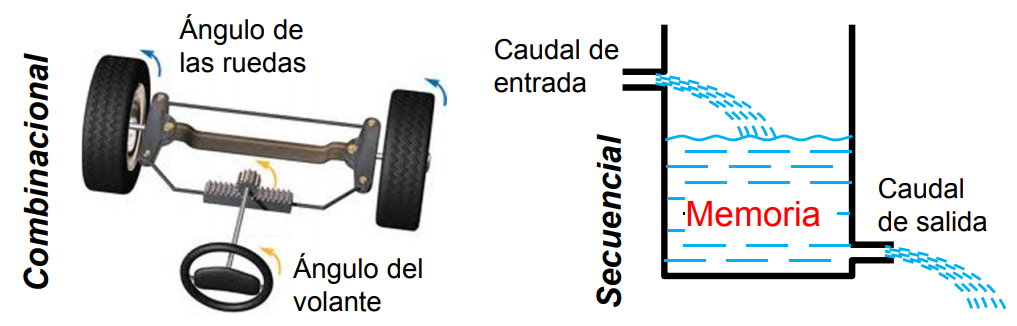
\includegraphics[scale=0.45]{secuencial y combinacional}
\end{center}

\begin{itemize}
\item \textbf{Síncronos}: las entradas y salidas solo pueden cambiar en un conjunto discreto de instantes definidos por una señal de reloj
\item \textbf{Asíncronos}: las entradas y salidas pueden cambiar en cualquier momento

\begin{center}
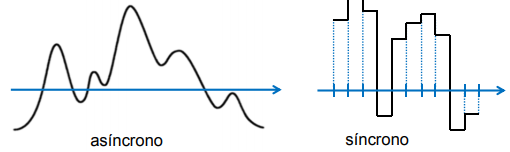
\includegraphics[scale=0.65]{sincrono y asincrono}
\end{center}

\end{itemize}

La \textbf{especificación} de un sistema es la descripción del comportamiento y funcionalidades que ese sistema posee (¿qué hace?).\par
La \textbf{implementación} de un sistema es la descripción en base al conjunto de elementos que forman ese sistema (¿cómo es?).

\section*{SISTEMAS DE NUMERACIÓN} 
Es un mecanismo que permite dar representación gráfica a cada número. Se define por:

\begin{itemize}
\item \textbf{Dígitos}: conjunto discreto de símbolos, lo que se conoce como la BASE
\item \textbf{Notación}: conjunto discreto de reglas de generación que permite representar números mayores a los dígitos
\item \textbf{Aritmética}: conjunto de reglas de manipulación de símbolos que permite realizar operaciones entre números coherentemente.
\end{itemize}

Además del sistema decimal, es posible utilizar el sistema binario, cuya base es 2, para expresar un número. El \textbf{sistema binario}, al igual que el decimal, es un sistema numérico POSICIONAL, es decir, en el que la posición del dígito influye en el valor del número en su totalidad.
El \textbf{sistema hexadecimal}, a su vez también es un sistema numérico posicional, pero cuya base numérica es 16. Se utiliza este sistema sobre todo por su correspondencia con 4 bits, lo que le aporta la capacidad de poder escribir grandes números binarios de forma abreviada.

\subsection*{\underline{Rango de representación}}
Con un número de $n$ dígitos decimales se pueden representar $10^n$ números distintos pertenecientes al rango: $(0,10^n-1)$
$$n=3\Rightarrow 10^3\mbox{ números distintos entre }(0,999)$$

Con un número de $n$ dígitos binarios se pueden representar $2^n$ números distintos pertenecientes al rango: $(0,2^n-1)$
$$n=3\Rightarrow 2^3\mbox{ números distintos entre }(0,7)$$

Con un número de $n$ dígitos hexadecimales se pueden representar $16^n$ números distintos pertenecientes al rango: $(0,16^n-1)$
$$n=3\Rightarrow 16^3\mbox{ números distintos entre }(0,4095)$$

\subsection*{\underline{Conversión entre sistemas}}
\begin{itemize}
\item $10^n\rightarrow 2^n$\par
Dividimos el número a convertir entre 2, 16, 8, …, anotamos el resto de la división y dividimos el cociente resultante hasta que este sea 1. Después, anotamos en orden inverso los sucesivos restos de las divisiones hasta INCLUIR el ÚLTIMO 1 DEL COCIENTE FINAL.
 
\begin{center}
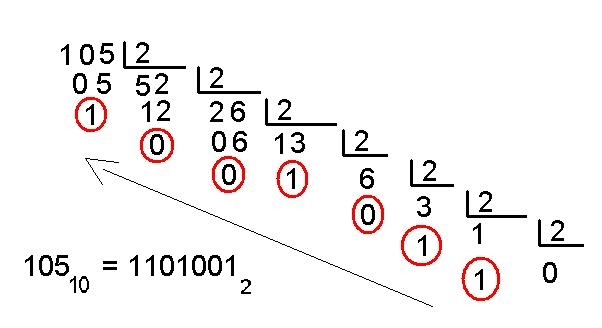
\includegraphics[scale=0.25]{decimal a binario}
\end{center}
 
\item $2^n,16^n,8^n,…\rightarrow 10^n$\par
Elevamos cada dígito a la potencia de $2^n,8^n,16^n,…$\footnote{De la utilización de dichos sistemas nace el término bit, byte y nibbles.} correspondiente siendo $x^0$ el dígito más a la derecha y $x^{n-1}$ el de más a la izquierda. El valor $n$ es el número de dígitos que tiene el valor binario.

\begin{center}
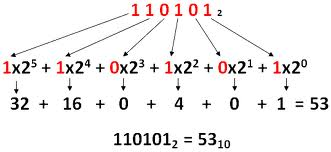
\includegraphics[scale=0.5]{pasar de binario a decimal}
\end{center}

\item $2^n\rightarrow 16^n, 8^n,...$\par
Se agrupan de derecha a izquierda los dígitos binarios de $i$ en $i$, siendo $i$: $base\mbox{ }R \rightarrow base\mbox{ }S=R^{i}$, es decir, $8=2^3\Rightarrow i=3, 16=2^4, i=4$ posteriormente se traduce el valor de ese dígito binario (que como máximo su cifra será 15 por lo explicado en el rango de representación) al dígito hexadecimal correspondiente:

\begin{center}
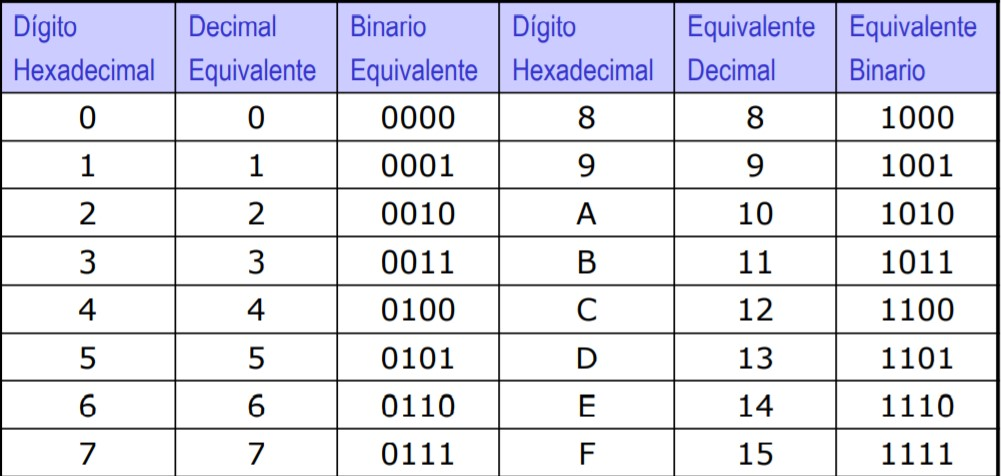
\includegraphics[scale=0.37]{correspondencia entre bin, dec y hex}
\end{center}

\item $16^n\rightarrow 2^n$\par
Mismo proceso, pero a la inversa.
\end{itemize}
\vspace{0.05cm}
\section*{REPRESENTACIÓN DE LA INFORMACIÓN}
Un sistema digital solo procesa información codificada en binario.\par
\textbf{Codificación}: es un convenio que asocia a cada elemento una representación en binario, por lo que un mismo elemento puede tener más de una representación en función de la codificación que se emplee.\par
Cada código emplea un número fijo de bits que limita el rango de representación de dicha codificación, cuando un número sobrepasa dicha frontera decimos que se produce un problema de desbordamiento o \textit{overfloat}, detectándose en un resultado incorrecto de las operaciones aritméticas realizadas.\par
\textbf{Para saber el número necesario de bits que hacen falta para representar un número, elegimos un $k:2^k-1>N$, siendo N mi número en decimal, después si existe bit de signo en nuestra codificación se escoge un $n=k+1$, siendo $k$ y $n$ el número de bits de nuestra codificación (en función de si tiene bits de signo o no}

\subsection*{\underline{Binario puro}}
Esta codificación solo representa números naturales.
\begin{itemize}
\item \textbf{Notación}: $k$ bits codifican la magnitud del natural
\item \textbf{Rango de representación}: $[0,2^k-1]$
\item \textbf{Aritmética}:
	\begin{itemize}
	\item Extensión: para pasar a mayor numero de bits completar con 0 por la izq.
	\item Suma: suma binaria normal, hay desbordamiento cuando al sumar los bits más significativos se produce acarreo
	\end{itemize}
\item \textbf{Proceso de codificación y decodificación}\par
Se siguen los pasos explicados en \textit{Conversión entre sistemas}
\end{itemize}

\subsection*{\underline{MyS}}
Esta codificación representa números enteros.
\begin{itemize}
\item \textbf{Notación}: 1 bit codifica el signo (0 es positivo y 1 es negativo) y $n-1$ bits codifican la magnitud del número.
\begin{itemize}
	\item Positivos: $+N_{10}\rightarrow 0(N)_2$
	\item Negativos: $-N_{10}\rightarrow 1(N)_2$
	\end{itemize}
\item \textbf{Rango de representación\footnote{El 0 posee doble representación (en negativo y positivo)}}: $\left[-(2^{n-1}-1),(2^{n-1}-1)\right]$
\item \textbf{Aritmética}:
	\begin{itemize}
	\item Cambio de signo: cambio del bit más significativo
	\item Extensión: para pasar a mayor numero de bits completar con 0 por la izq. conservando el primer bit intacto (bit de signo).
	\item Suma y Resta
	\end{itemize}
\item \textbf{Proceso de codificación y decodificación}\par
Para \textbf{codificar}, primero se codifica la magnitud de la forma explicada en \textit{Conversión entre sistemas} y después se le agrega a la izquierda el bit de signo correspondiente.\par
Para \textbf{decodificar} el número, primero se decodifica el bit de signo y con los $n-1$ bits restantes se decodifica la magnitud.
\end{itemize}

\subsection*{\underline{Complemento a 2}}
Esta codificación representa números enteros.
\begin{itemize}
\item \textbf{Notación}:
	\begin{itemize}
	\item Positivos: $+N_{10}\rightarrow 0(N)_2$
	$$12_{10}\rightarrow 01100_{C2}$$
	\item Negativos: $-N_{10}\rightarrow (2^n-N)_2=C2(N_2)$
	$$-12_{10}\rightarrow 2^5-12=20 \rightarrow 10100_{C2}$$
	\end{itemize}
\item \textbf{Rango de representación\footnote{El 0 ahora posee una única representación y el rango de representación es asimétrico (hay un negativo más)}}: $[-2^{n-1},+2^{n-1}-1]$
\item \textbf{Aritmética\footnote{Cuando el bit de signo de los sumandos y del resultado coincide NO hay desbordamiento, cuando se suman número de distinto signo NUNCA hay desbordamiento}}:
	\begin{itemize}
	\item Cambio de signo: hacer el complemento a 2 del número. Formas:
		\begin{itemize}
	\item Hacer un NOT a todos los bits y sumarle uno a ese número.
$$12_{10}=01100_2 \rightarrow 10011 \rightarrow 10011+1 \rightarrow 10100_{C2}=-12_{10}$$
	\item Recorrer el número de derecha a izquierda hasta encontrar un 1 y a partir de él invertir los demás bits restantes.
$$12_{10}=01100_2 \rightarrow 10100_{C2}=-12_{10}$$
		\end{itemize}			

	\item Extensión: replicar el bit más significativo hacia la izquierda.
	\item Suma: suma binaria, \textbf{NO se tiene en cuenta acarreo del bit más significativo}
	\item Resta: se suele expresar como suma del opuesto, es decir, del complementado a dos del sustraendo.
	\end{itemize}
\item \textbf{Proceso de codificación y decodificación}\par
Para \textbf{codificar} un \emph{número positivo} se siguen las reglas comentadas en el punto \textit{Conversión entre sistemas}. Para \emph{números negativos} se convierte como si fuese positivo y se realiza el complemento a 2 del resultado.\par
Para \textbf{decodificar}, para \emph{números positivos}, decodificar como en \textit{Conversión entre sistemas}. Para \emph{números negativos}, hacer su complemento a 2 y decodificar como los positivos, añadiéndole después el signo.
\end{itemize}

\subsection*{\underline{Complemento a 1}}
Esta codificación representa números enteros.
\begin{itemize}
\item \textbf{Notación}:
\begin{itemize}
	\item Positivos: $+N_{10}\rightarrow 0(N)_2$
	\item Negativos: $-N_{10}\rightarrow (2^n-1-N)_2=C1(N_2)$
$$-12_{10}\rightarrow 2^5-1-12=19 \rightarrow 10011_{C1}$$
	\end{itemize}
\item \textbf{Rango de representación\footnote{El 0 posee doble representación}}: $[-(2^{n-1}-1),+(2^{n-1}-1)]$
\item \textbf{Aritmética\footnote{Cuando el bit de signo de los sumandos y del resultado coincide NO hay desbordamiento, cuando se suman número de distinto signo NUNCA hay desbordamiento}}:
	\begin{itemize}
	\item Cambio de signo: hacer el complemento a 1 del número. Formas:
		\begin{itemize}
		\item Hacer un NOT a todos los bits
				$$12_{10}=01100_2 \rightarrow 10011_{C1}$$
		\end{itemize}
	\item Extensión: replicar el bit más significativo hacia la izquierda.
	\item Suma: suma binaria, \textbf{NO se tiene en cuenta acarreo del bit más significativo}
	\item Resta: se suele expresar como suma del opuesto, es decir, del complementado a dos del sustraendo.
	\end{itemize}
\item \textbf{Proceso de codificación y decodificación}\par
Para \textbf{codificar} un \emph{número positivo} se siguen las reglas comentadas en el punto \textit{Conversión entre sistemas}. Para \emph{números negativos} se convierte como si fuese positivo y se realiza el complemento a 1 del resultado.\par
Para \textbf{decodificar}, para \emph{números positivos}, decodificar como en \textit{Conversión entre sistemas}. Para \emph{números negativos}, hacer su complemento a 1 y decodificar como los positivos, añadiéndole después el signo.
\end{itemize}
\begin{center}
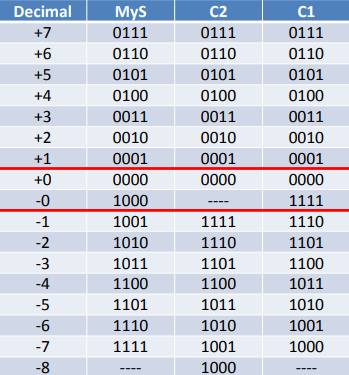
\includegraphics[scale=0.75]{comparacion de codigos}
\end{center}

Existen otros métodos de representación en binario como el \textbf{BCD} o el \textbf{Exceso\footnote{El método de exceso 3 es igual que BCD, pero sumando a la cifra 3 unidades} 3} que codifican cada cifra por separado en grupos de 4 dígitos binarios:
$$375_2\rightarrow 0011|0111|0101\rightarrow 001101110101_{BCD}$$
$$375_2\rightarrow 0110|1010|1000\rightarrow 011010101000_{EX-3}$$

\chapter*{ESPECIFICACIÓN DE SISTEMAS COMBINACIONALES}
En este tema nos centramos en hallar la función que describe el comportamiento de esa ``caja negra'' que es nuestro sistema, es decir, de la foto de abajo hallar la función \textbf{F} que describe Z(t):

\begin{center}
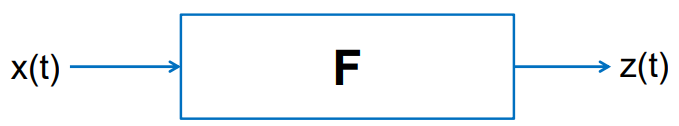
\includegraphics[scale=0.35]{sistema digital}
\end{center}

Para ello tendremos que describir:
\begin{itemize}
\item Valores de entrada $\rightarrow$ Dominio 
\item Salidas $\rightarrow$ Codominio
\item Función: trabaja con los valores
\end{itemize}
\section*{ESPECIFICACIÓN DE ALTO NIVEL}
En un primer momento procederemos a realizar una especificación de alto nivel, esto quiere decir, determinar los valores de entrada y salida que puede tomar nuestro sistema y el comportamiento lógico que la función debe tener a la hora de transformar nuestros valores:\par
Ej.:
\begin{itemize}
\item $x(t)=\{0,1,2,3\}$
\item $z(t)=\{0,1,2,...,7\}$
\item $f(t)=2\cdot x(t)+1$
\end{itemize}

Ej.:
\begin{center}
\begin{tabular}{|c|c|c|c|c|c|c|c|c|}
\hline
 x & 0 & 1 & 2 & 3 & 4 & 5 & 6 & 7 \\
 \hline
 z & 0 & 1 & 2 & 0 & 1 & 2 & 0 & 1 \\
 \hline  
\end{tabular}\par
\end{center}

Ej.:
\begin{equation*}
\begin{cases}
1 & \mbox{si } x(t)\mbox{ es primo} \\
0 & \mbox{si } x(t)\mbox{ no es primo }\\
\end{cases}
\end{equation*}

Sin embargo, para poder trabajar con estas expresiones es necesario codificarlas en alguna codificación binaria. Esto nos da como resultado en vez de entrada \textit{x}, un vector de entrada \textit{x} de \textit{n} bits, siendo \textit{n} el mínimo necesario para expresar todos los valores de entrada\footnote{Expresar todos los valores de entrada no quiere decir expresar su magnitud en binario sino asociarle un número en binario que lo represente por lo que n tendrá que ver con la cantidad de valores de entrada, no con la magnitud que representen dichos valores}.
$$x: (x_{n-1}, ..., x_0)$$
Del mismo modo ocurre con la cantidad de valores de salida que ahora pasa a ser un vector de \textit{m} bits\footnote{No es necesario que \textit{m} y \textit{n} coincidan}, siendo \textit{m} el mínimo necesario para codificar todas las posibles combinaciones de salida.
$$z: (z_{m-1}, ..., z_0)$$
Y existirán \textit{m} funciones de salida para codificar una a cada bit de salida y que trabajaran con los \textit{n} bits de entrada.
$$F=(f_{m-1},..., f_0): f_i=\{0,1\}\rightarrow z_i : i=(0,m-1)$$
Es decir, representando cada bit en una tabla\footnote{Los valores de z en este caso son aleatorios, debería ser los valores discretos que tomasen mis sistemas en realidad} con valores como $m=3$ y $n=2$ :

\begin{center}
\begin{tabular}{|c|c|c|c|c|}
\hline
 $x_1$ & $x_0$ & $z_1$ & $z_2$ & $z_3$ \\
 \hline
 0 & 0 & 0 & 1 & 1 \\
 \hline
 0 & 1 & 1 & 1 & 0 \\
 \hline  
 1 & 0 & 1 & 0 & 0 \\
 \hline  
 1 & 1 & 0 & 1 & 0 \\
 \hline  
\end{tabular}\par
\end{center}

En ocasiones las funciones no están completamente especificadas y decimos que están \textbf{parcialmente especificadas}. En estos casos los valores de entrada para los que no hay salida especificada se marcan con un ``$-$'' en la casilla de la salida correspondiente a la entrada sin asignación.

\section*{FUNCIONES DE CONMUTACIÓN}
Una función de conmutación es una función que asocia un conjunto de \textit{n} 0 y 1 a otro conjunto de 0 y 1.
$$f: {0,1}^n \longmapsto {0,1}$$
El número de funciones que existen para \textit{n} variables es $2^{2n}$
\begin{center}
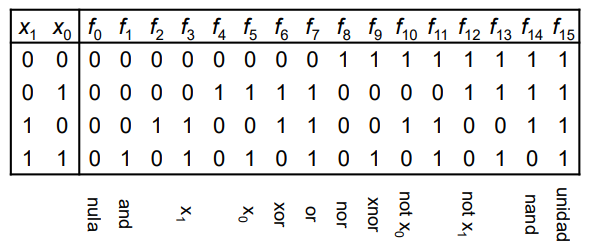
\includegraphics[scale=0.75]{tabla funcion}
\end{center}
En ocasiones estas están incompletamente especificadas y asocian el valor ``-'' a su salida.
\subsection*{\underline{Expresiones de conmutación}}
Para representar estas funciones de forma más compacta, manipulable y sintetizable se emplean las expresiones de computación o EC.
$$F=\bar{A}+CD+[B\cdot(A+C)]$$
Estas son fórmulas que describen el comportamiento de la función, en función de los valores de las variables lógicas de entrada y que se rigen por las Leyes del Álgebra de Boole:

\subsubsection*{Leyes del Álgebra de Boole}
\begin{enumerate}
\item \textbf{Ley de la dualidad}: cualquier expresión o identidad en el álgebra de Boole tiene su expresión dual intercambiando el $+$ por la $\cdot$ y los 0 por los 1.

\item \textbf{Teorema de la identidad}: $B\cdot1=B$\par
\textbf{Dual de la identidad}: $B+0=B$

\item \textbf{Teorema del elemento nulo}: $B\cdot 0=0$\par
\textbf{Dual de elemento nulo}: $B+1=1$
 
\item \textbf{Teorema de la potencia}: $B\cdot B=B$\par
\textbf{Dual de la potencia}: $B+B=B$  

\item \textbf{Teorema de la involución}: $\bar{\bar{B}}=B$

\item \textbf{Teorema del complemento}: $B\cdot \bar{B}=0$\par
\textbf{Dual del complemento}: $B+\bar{B}=1$

\item \textbf{Teorema de la propiedad conmutativa}: $B\cdot C=C\cdot B$\par
\textbf{Dual de la propiedad conmutativa}: $B+C=C+B$

\item \textbf{Teorema de la propiedad asociativa\footnote{Quiere decir que el resultado de la aplicación de las dos puertas AND es el mismo que el de la aplicación de una única puerta AND de 3 entradas.}}: $(B\cdot C)\cdot D=B\cdot (C\cdot D)$\par
\textbf{Dual de la propiedad asociativa\footnote{Quiere decir que el resultado de la aplicación de las dos puertas OR es el mismo que el de la aplicación de una única puerta OR de 3 entradas.
 }}: $(B+C)+D=B+(C+D)$

\item \textbf{Teorema de la propiedad distributiva}:$(B\cdot C)+(B\cdot D)=B(C+D)$\par
\textbf{Dual de la propiedad distributiva}: $(B+C)\cdot (B+D)=B+(C\cdot D)$ 

\item \textbf{Ley de Morgan}: $\overline{x\cdot y}=\bar{x}+\bar{y}$\par
\textbf{Dual de la Ley de Morgan}:$\overline{x+y}=\bar{x}\cdot\bar{y}$ 
\end{enumerate}

\subsubsection*{Valores de una EC}
El valor de una EC para una combinación de entrada o asignación concreta se expresa como:
$$v(E,a)$$
Ej.: $E=A+\bar{B}C+B$, $a=(0,1,1)$
$$v(E,a)=v(A+\bar{B}C+B, (0,1,1))= 0+0\cdot 1 + 1=1$$

\subsubsection*{Suma de productos}
Cualquier expresión de conmutación puede ser descrita como suma de mintérminos. Estos se corresponden a cada fila de la tabla de verdad y constituyen un producto (AND) de las variables y sus complementarias.
\begin{enumerate}
\item Recogemos en una tabla de verdad todo los posibles casos de entrada y las SALIDAS CORRESPONDIENTES POR OBSERVACIÓN EMPÍRICA (no tenemos por qué saber el porqué de esas salidas).
\item Escribimos en la tabla de los mintérminoss el correspondiente en función de los valores de A y de B, siendo el mintérminos un producto de ambas variables y cada variable ser A, si vale 1 en la tabla de verdad, o $\bar{A}$ si su valor es un 0.
\item La función se construye solo con la SUMA DE MINTÉRMINOS VERDADEROS, que son los que están en una fila donde la salida sea 1.
\end{enumerate}

\begin{center}
\footnote{Se ha puesto el símbolo ¬ por confusión del signo $\bar{}$ con las líneas}
\begin{tabular}{|c|c|c|c|}
\hline
A & B & F & Mintérmino \\
\hline
0 & 0 & 0 & $\neg A\cdot \neg B$ \\
\hline
0 & 1 & 1 & $\neg A \cdot B $ \\
\hline
1 & 0 & 0 & $A\cdot \neg B $ \\
\hline
1 & 1 & 1 & $A\cdot B$ \\
\hline
\end{tabular}
\end{center}
Ej.:
$$F=\sum m(1,3)=\bar{A} \cdot B + A\cdot B$$

\subsection*{\underline {Simplificación de EC}}
\subsubsection*{Simplificación algebraica}
Se trata de simplificar una EC dada usando las leyes básicas del álgebra de boole:
\begin{enumerate}
\item Pasar de una expresión cualquiera a una SPC

Para pasar de una expresión simplificada a una SPC, damos TODOS los valores posibles a las variables que no están en los mintérminos simplificados.\par
Ej.:
$$f(x,y,z,w)=\bar{y}z+y\bar{z}\Rightarrow
\begin{cases}
\bar{y}z & =\bar{x}\bar{y}z\bar{w}+ \bar{x}\bar{y}zw=x\bar{y}z\bar{w}+x\bar{y}zw \\
y\bar{z} & =\bar{x}y\bar{z}\bar{w}+ \bar{x}y\bar{z}w + xy\bar{z}\bar{w}+ xy\bar{z}w
\end{cases}
\Rightarrow  f(x,y,z,w)=\sum m(2,3,4,5,10,11,12,13)
$$

\item Simplificar dicha SPC usando las reglas de las leyes de conmutación (las variables que cambien entre minterms con variables comunes se simplificaran al final del proceso)

\end{enumerate}

\subsubsection*{Mapas de Karnaugh}
Para facilitar la realización de este proceso utilizando la mínima cantidad de recursos posibles (cuantos menos términos menores puertas lógicas) usamos los Diagramas de Karnaugh.\par
Se tratan de una secuencia de celdas, en la que cada celda representa un valor binario de las diferentes entradas. Además, cada celda contiene dentro de ella el valor de salida correspondiente a la combinación de entrada que representa dicha celda en la tabla de verdad.\par
Es muy importante distribuir las celdas de forma que SOLO SE DIFERENCIEN EN 1 BIT, por ello es por lo que en el dibujo se han cambiado las dos últimas celdas. Pueden usarse para expresiones de como MÁXIMO 6 variables y para n variables, es necesario utilizar $2^n$ celdas.

\begin{center}
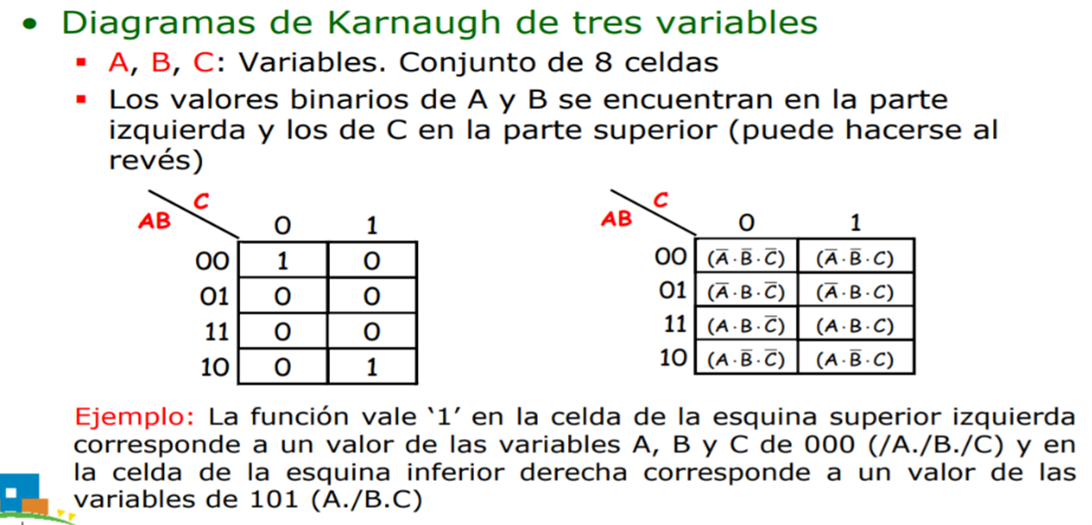
\includegraphics[scale=0.75]{mapas 1}
\end{center}

\begin{center}
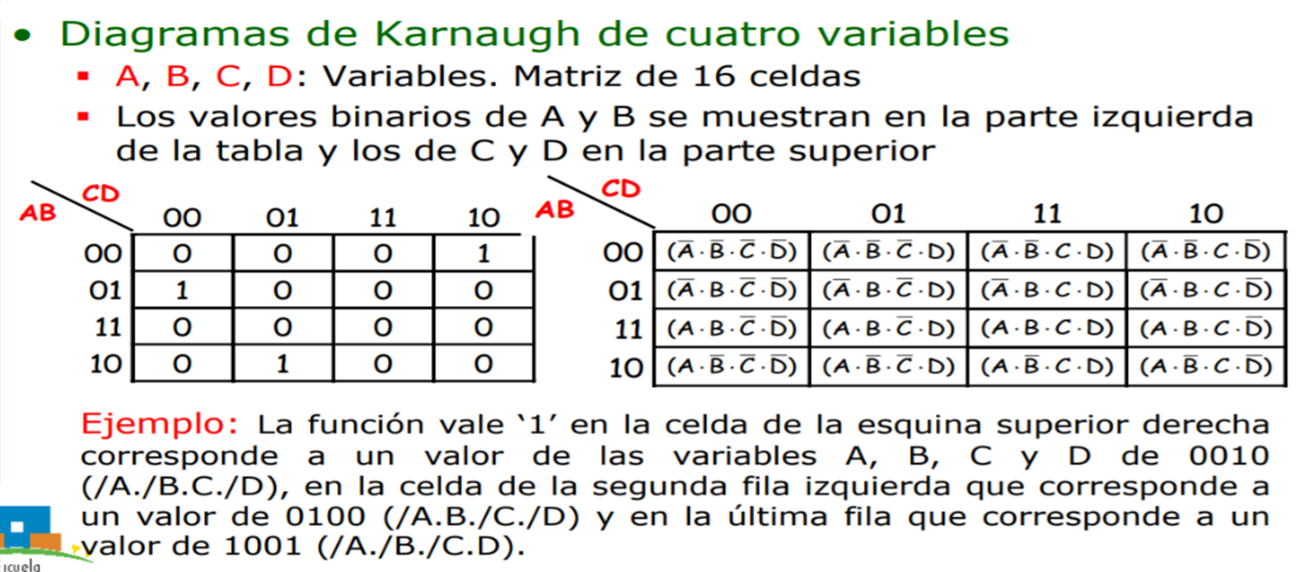
\includegraphics[scale=0.75]{mapas 2}
\end{center}

\begin{center}
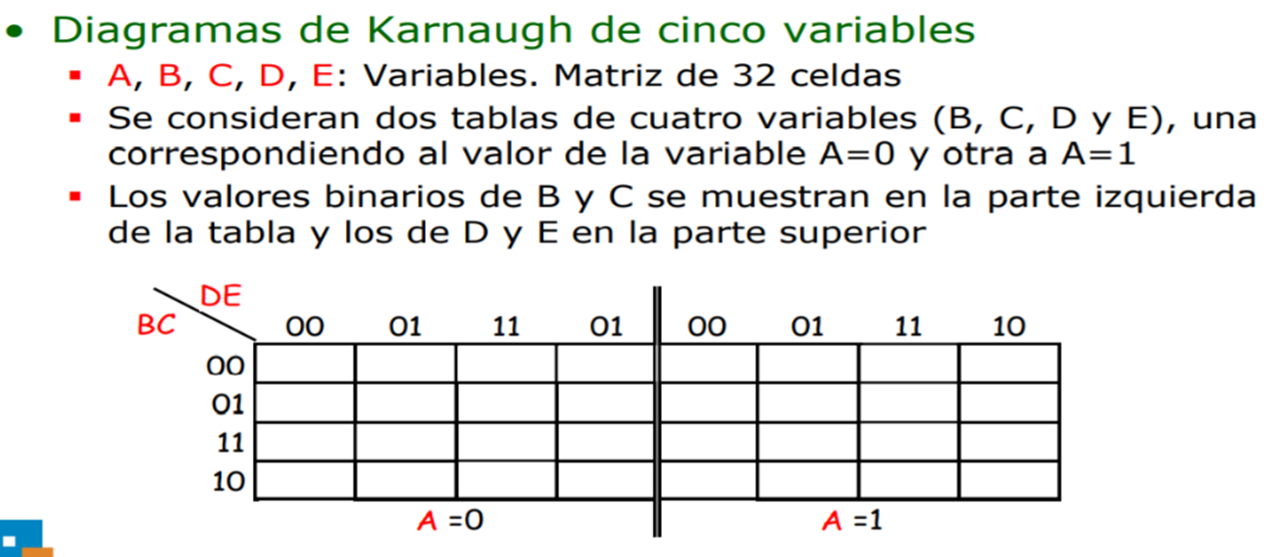
\includegraphics[scale=0.75]{mapas 3}
\end{center}

Los mapas de Karnaugh no se usan únicamente como una forma condensada de una tabla de verdad, sino que además permiten por su disposición la MINIMIZACIÓN de la expresión resultante. Para ello es importante tener claro el concepto de adyacencia y las condiciones de formación de grupo:
\begin{enumerate}
\item Entre celdas adyacentes solo cambia una variable, es decir, un bit.
\item Solo se consideran adyacentes las que estén situadas inmediatamente por cualquier lado.
\item Las celdas en diagonal no son adyacentes.
\item Las celdas siguen ADYACENCIA CÍCLICA, las del borde de la izquierda lo son con las de la derecha y las del borde de arriba con el de abajo.
\end{enumerate}

Para realizar esta minimización es necesario traducir de Minterms o Maxterms a mapa de Karnaugh si tenemos solo la expresión de la función que se quiere reducir $(F=ABC+...)$ o simplemente proporcionar el valor 0 o 1 de la tabla de verdad en la combinación de entradas correspondiente:

\begin{center}
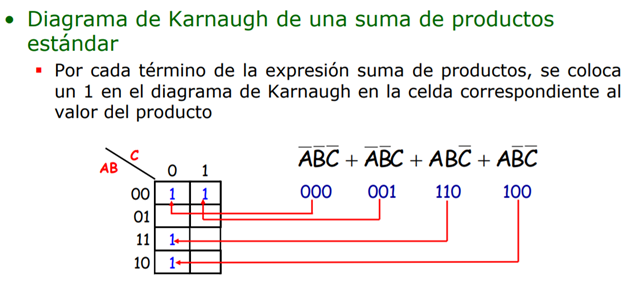
\includegraphics[scale=0.95]{mapas 4}
\end{center}

La agrupación de 1 o 0 se hace en base a las siguientes normas:
\begin{itemize}
\item Cada grupo debe contener un número de unos correspondiente a un múltiplo de 2 (los grupos siempre serán rectangulitos o cuadrados)
\item Cada celda del grupo debe ser adyacente a una o más celdas del grupo
\item Todos los 1 o 0 deben estar en algún grupo y los grupos deben tener el máximo de ellos, aunque un elemento este en varios grupos.
\end{itemize}

\begin{center}
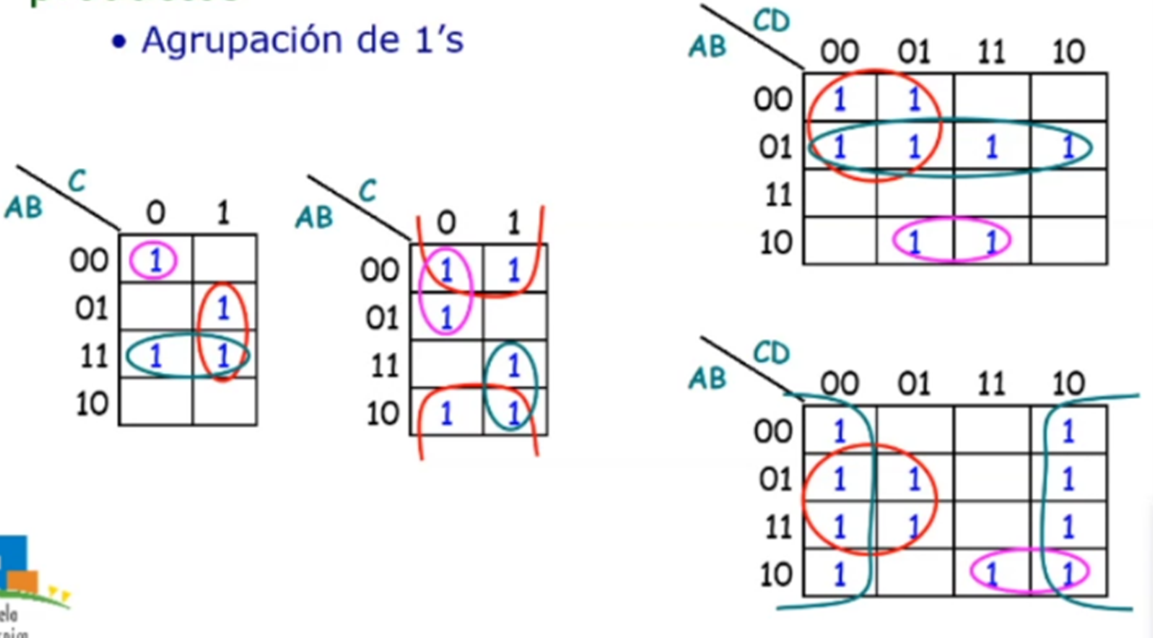
\includegraphics[scale=0.95]{mapas 5}
\end{center}

Una vez agrupados los términos de la forma correspondiente:
\begin{itemize}
\item Cada grupo constituye un producto de todas las variables que posteriormente se sumará a los demás
\item En un mismo grupo, SOLO SE MANTIENEN las variables que NO VARÍAN
\item Se escribe como $\bar{A}$ o como A la variable en función de si vale 1 (minterms) o 0 (maxterms)
\end{itemize}

Para los mapas de 5 variables, las normas son las mismas con la peculiaridad de colocar uno encima del otro:

\begin{center}
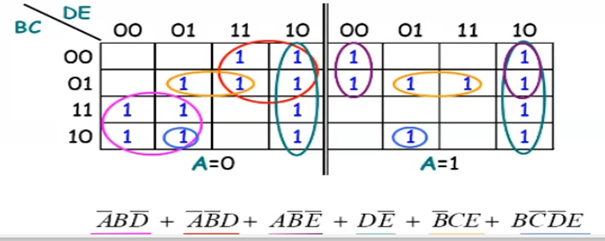
\includegraphics[scale=0.95]{mapas 6}
\end{center}

\begin{center}
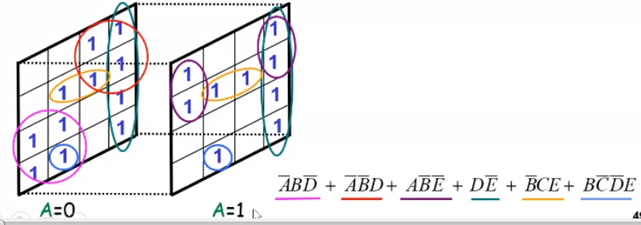
\includegraphics[scale=0.95]{mapas 7}
\end{center}


\chapter*{IMPLEMENTACIÓN DE SISTEMAS COMBINACIONALES}
\section*{PUERTAS LÓGICAS}
Son elementos lógicos digitales a partir de los cuales se crean funciones lógicas de forma física:
\begin{itemize}
\item \textbf{BUFFER o Amplificador} $\rightarrow$ Los datos de entrada son los mismos que los de salida.
	\begin{itemize}
	\item Buffer triestado: posee una variable auxiliar ``enable'' que habilita o no el buffer.
	\end{itemize}
	
\begin{center}
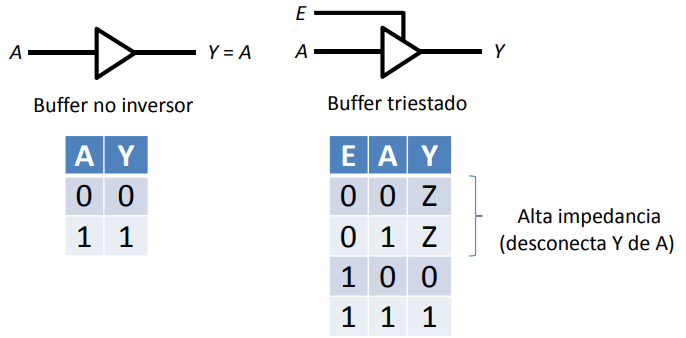
\includegraphics[scale=0.45]{buffer triestado}
\end{center}	
	
\item \textbf{NOT o Inversor} $\rightarrow$ Los datos de entrada son contrarios a los de salida.
\item \textbf{AND o Multiplicación Lógica} $\rightarrow$ La salida solo vale uno si ambas entradas valen 1.
\item \textbf{OR o Suma Lógica} $\rightarrow$ La salida vale 1 si al menos uno de los datos de entrada vale 1 (o todos).
\item \textbf{NAND} $\rightarrow$ Funciona como una puerta AND, pero al resultado se le aplica el NOT.
\item \textbf{NOR} $\rightarrow$ Funciona como una puerta OR, pero al resultado se le aplica el NOT.
\item \textbf{XOR} $\rightarrow$ Es como la puerta OR, pero excluyente: la salida es 1 si solo una de sus entradas vale 1.
\item \textbf{XNOR} $\rightarrow$ Es como la puerta XOR, pero cuando solo una de sus entradas vale 0 su salida vale 0.
\end{itemize}

\begin{center}
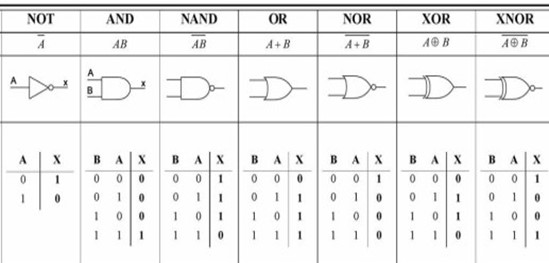
\includegraphics[scale=0.75]{puertas logicas}
\end{center}

No es necesario que las puertas tengan únicamente dos entradas, sino que pueden ser las que queramos, aunque en la práctica es habitual encontrar un número elevado de ellas. En lugar de ello se recurre a la implementación en árbol:

\begin{center}
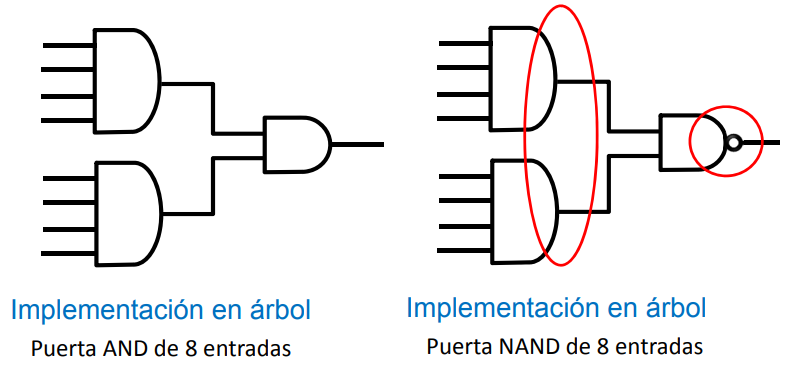
\includegraphics[scale=0.5]{imp arbol}
\end{center}

Existen a su vez puertas compuestas homologadas como:

\begin{center}
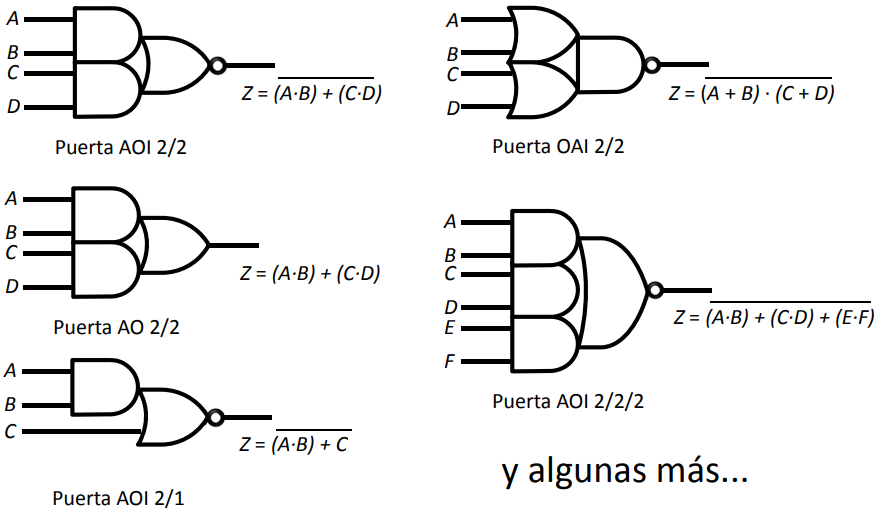
\includegraphics[scale=0.5]{puertas compuestas}
\end{center}

\subsection*{\underline {Definiciones}}
\begin{itemize}
\item \textbf{\large{Módulo}}: dispositivo que realiza físicamente una función conocida de cualquier complejidad. Ej.: Puertas lógicas, microchips, memorias RAM...
\item \textbf{\large{Puerto}}: cada línea de entrada o salida que comunica el módulo con el exterior.
\item \textbf{\large{Interconexión}}: unión de dos o más puertos entre sí.
Notación:

\begin{center}
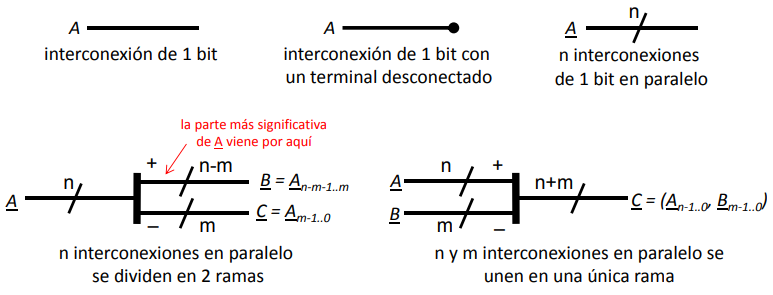
\includegraphics[scale=0.65]{interconexiones}
\end{center}

\item \textbf{\large{Red}}: colección de módulos interconectados de manera que toda ENTRADA SOLO VIENE de UNA SALIDA. (Una salida si puede estar conectada a más de una entrada).
\item \textbf{\large{Red combinacional}}: red de módulos combinacionales en las que no hay retroalimentaciones (porque hay sistemas secuenciales implementados con módulos combinacionales), es decir, que ningún recorrido de la red pasa por el mismo punto dos veces.
\item \textbf{\large{Nivel de una red}}: número máximo de módulos que atraviesa cualquier camino que conecta una entrada con una salida. (Cuando la red es de puertas no solemos contar con los inversores).
\end{itemize}

\subsection*{\underline{Conjunto Universal}}
Decimos que un conjunto de módulos combinacionales es universal cuando permite implementar cualquier fórmula empleando sólo dichos módulos:
Ej.:
\begin{itemize}
\item \{AND, NOT, OR\}
$$a+b=\overline{\overline{a+b}}=\overline{\bar{a}\cdot \bar{b}}$$
\item \{NAND\}
$$\bar{a}=\overline{a\cdot a}$$
$$a\cdot b=\overline{\overline{a\cdot b}}$$
$$a+b=\overline{\overline{a+b}}=\overline{\bar{a}\cdot \bar{b}}$$
\item \{OR, NOT\}, \{NOR\}, \{XOR, AND\}, ...
\end{itemize}

\section*{SÍNTESIS DE REDES DE PUERTAS}
El proceso de automatización de la descripción de un proceso lógico termina con la implementación en un circuito de la expresión booleana resultante, es decir, para crear un sistema físico que describa el comportamiento de mi función lógica seguimos estos pasos:
\begin{enumerate}
\item Especificación de alto nivel
\item Codificación binaria de la especificación hecha
\item Simplificación de la codificación a una EC simplificada
\item Implementación del circuito por medio de las puertas lógicas
\end{enumerate}
Dentro de este último paso conocemos dos implementaciones posibles distintas:
\begin{itemize}
\item \textbf{Implementación a dos niveles}
\begin{itemize}
\item Implementación canónica: implementa la SPC
\item Implementación mínima: implementa la EC simplificada
\end{itemize}

\begin{center}
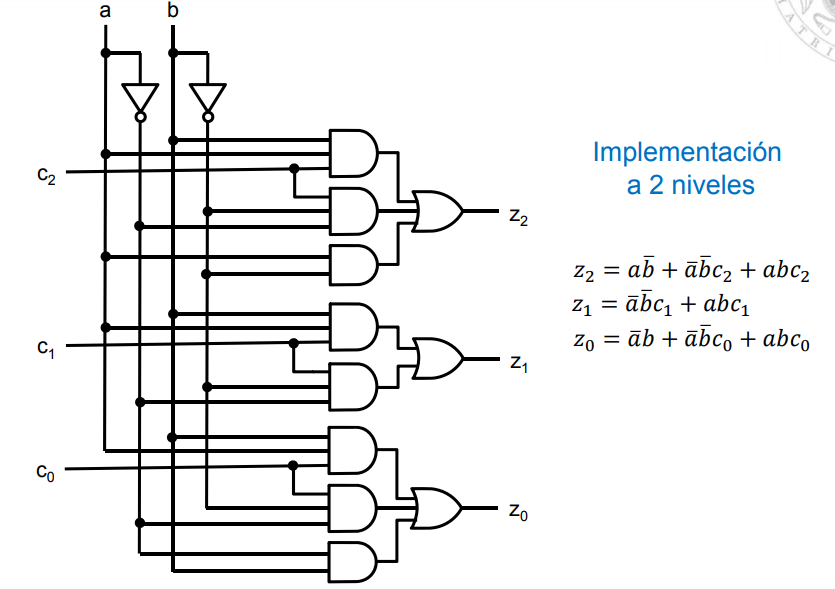
\includegraphics[scale=0.35]{imp multinivel}
\end{center}

\item \textbf{Implementación multinivel}: se realiza una simplificación heurística de la EC

\begin{center}
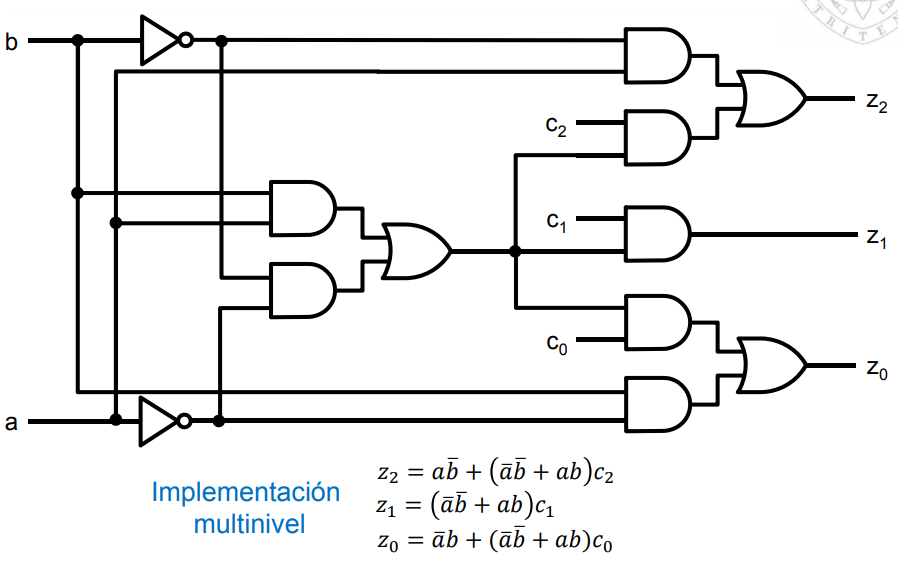
\includegraphics[scale=0.35]{imp dos niveles}
\end{center}
\end{itemize}

Para realizar la implementación de un circuito con el empleo exclusivo de puertas NAND, se sigue el siguiente procedimiento:

\begin{center}
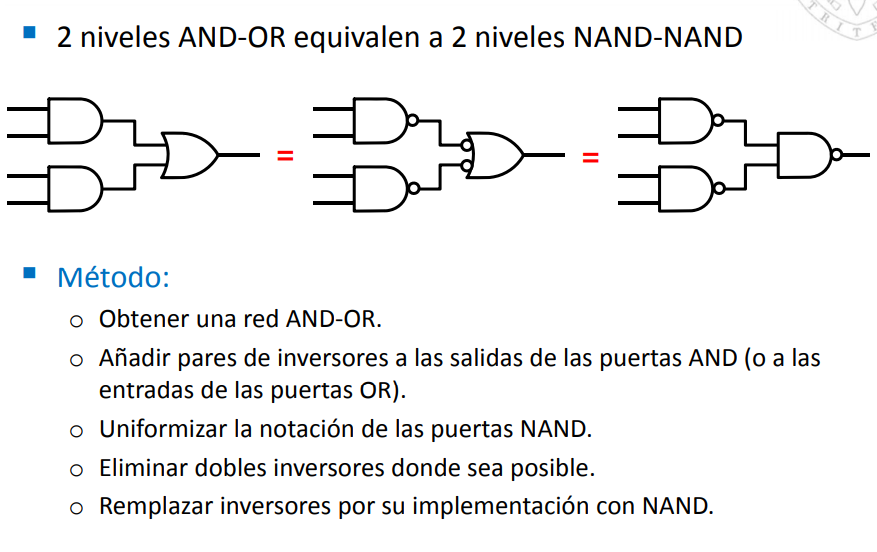
\includegraphics[scale=0.35]{imp en NAND}
\end{center}

Concretamente, para las expresiones de conmutacion, la expresion se transforma negando dos veces la expresion resultante y transformando de la siguiente forma:

\section*{ANÁLISIS DE REDES DE PUERTAS}
En ocasiones, nuestro trabajo no es implementar un circuito sino deducir la EC que un circuito ha implementado, para ello se siguen los siguientes pasos:
\begin{enumerate}
\item Asignar una variable a cada una de las interconexiones
\item Calcular la EC de cada una de esas variables
\item Sustituir su valor en las sucesivas EC hasta obtener una única EC
\item Simplificar dicha expresión
\end{enumerate}

\begin{center}
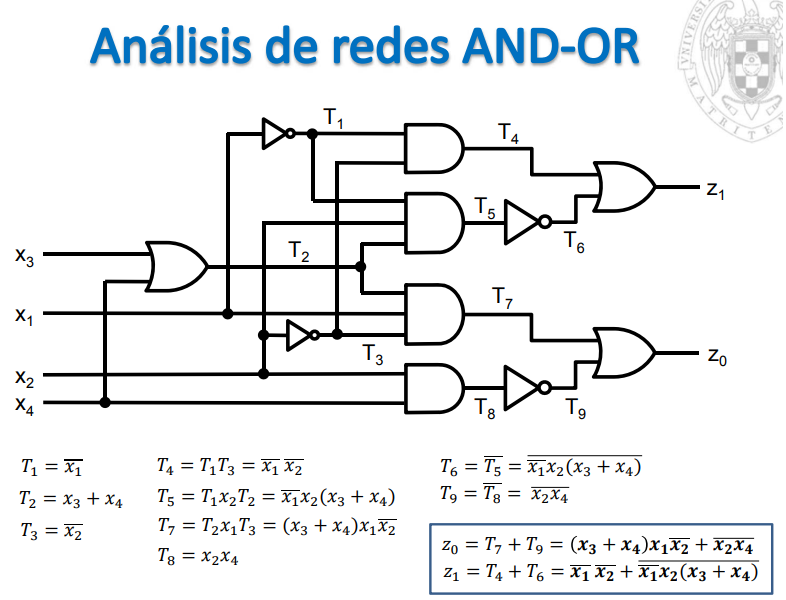
\includegraphics[scale=0.45]{analisis puertas}
\end{center}


\chapter*{MÓDULOS COMBINACIONALES}
En este tema estudiaremos los diferentes módulos combinacionales más básicos y su funcionamiento elemental. En ocasiones, el uso de puertas lógicas para implementación de funciones de conmutación se vuelve engorroso y muy complejo, fruto de facilitar y automatizar dicho trabajo nacen los módulos combinacionales, cuya funcionalidad es la implementación de funciones más complejas con métodos más mecánicos y versátiles (puesto que los módulos son piezas de lego ya definidas y combinables, es decir, más escalables).

\subsection*{\underline{Decodificador}}
Es un módulo combinacional con las siguientes características:
\begin{itemize}
\item Posee $n$ entradas y $2^n$ salidas.
\item El valor de la salida se define\footnote{Llamamos $v$ al valor del decimal de la entrada codificada en binario.} \footnote{Llamamos $z_i$ al bit del vector de salida que se activa cuando la entrada es concreta.} de la siguiente forma:
\begin{gather}
(v)_{10}=(x_0,x_1,..., x_n)_2 \\
z_i=\begin{cases} 1 &\mbox{ si }v=i \\ 0 &\mbox{ si }v\neq i \end{cases}
\end{gather}
\item Puede poseer o no una entrada de control llamada \textit{enable}, que cuando vale 0 convierte todos los bits de salida en 0 y cuando vale 1 sigue la disposición nombrada antes.
\end{itemize}

El símbolo empleado para denotar a un decodificador es:
\begin{center}
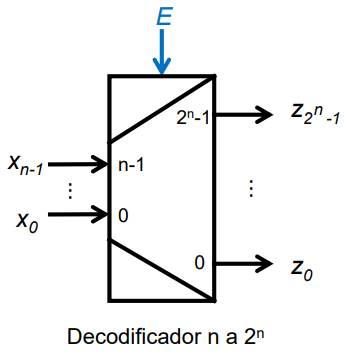
\includegraphics[scale=0.65]{deco}
\end{center}
Es decir, cuando el número decimal de entrada es el $x$, entonces la salida $z_x$ se activa y el resto distintas a esa salida no, si existe un enable, es como si este ``apagara'' o encendiese el módulo, cuando vale 0 no funciona.\par

Veamos un ejemplo de implementación de un decodificador de 2 entradas y 4 salidas con Enable. La implementación directa de puertas AND quedaría de la siguiente forma:
\begin{multicols}{2}
\begin{center}
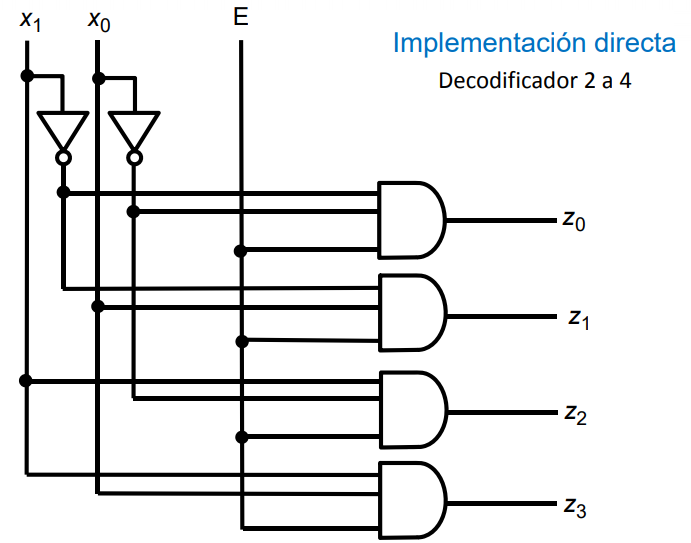
\includegraphics[scale=0.45]{deco2}
\end{center}

\begin{center}
\begin{tabular}{|c|c|c|c|c|c|c|}
\hline
$E$ & $x_0$ & $x_1$ & $z_0$ & $z_1$ & $z_2$ & $z_3$ \\
\hline
0 & 0 & 0 & 0 & 0 & 0 & 0 \\
\hline
0 & 0 & 1 & 0 & 0 & 0 & 0 \\
\hline
0 & 1 & 0 & 0 & 0 & 0 & 0 \\
\hline
0 & 1 & 1 & 0 & 0 & 0 & 0 \\
\hline
1 & 0 & 0 & 1 & 0 & 0 & 0 \\
\hline
1 & 0 & 1 & 0 & 1 & 0 & 0 \\
\hline
1 & 1 & 0 & 0 & 0 & 1 & 0 \\
\hline
1 & 1 & 1 & 0 & 0 & 0 & 1 \\
\hline
\end{tabular}
\end{center}
\end{multicols}

Estos módulos se pueden combinar entre sí para implementar otro del mismo tipo pero con mayor número de entradas, lo que le confiere la ventaja de escalabilidad característica de los módulos combinacionales, por ejemplo:
\begin{center}
\includegraphics[scale=0.65]{Deco16}
\end{center}

\subsubsection*{Aplicaciones de diseño}
Se puede observar que un decodificador de $n$ entradas posee $2^n$ salidas y, en consecuencia, se ve que cada puerta \textit{AND} conectada a una de las salidas permite implementar todos cada minterm de una función de conmutación concreta.\par
Dicho esto uno puede pensar que si el decodificador implementa todos los minterms y cualquier función de conmutación se puede escribir como \textit{Suma de Productos Canónica}, entonces si utilizamos unas puertas \textit{OR} para decidir qué minterms implementar y cuáles no, ya tendríamos la posibilidad de implementar cualquier FC de $n$ variables.

\begin{center}
\includegraphics[scale=0.23]{aplicaciones diseño deco}
\end{center}

Es decir, suele resultar útil para implementar funciones con $m$ salidas dependientes de $n$ entradas porque cada salida del decodificador implementa un minterm y \textbf{una puerta \textit{OR}} por cada salida $m$ implementa la suma de minterms de cada salida.


\subsection*{\underline{Codificador}}
Realiza la función contraria al decodificador, en este caso:
\begin{itemize}
\item Posee $2^n$ entradas y $n$ salidas.
\item El valor de la salida se define de la siguiente forma:
$$Z=(z_0,...,z_n)_{2}=(i)_2: x_i=1$$
\item \textbf{Siempre} debe tener una entrada de control llamada \textit{enable}, que cuando vale 0 inhabilita la salida.\footnote{Es fácil ver que para la codificación de entrada de todo 0, se puede confundir con la que está solo $x_0$ activada}
\item Posee una salida adicional, \textbf{la salida de actividad} $A$ que indica si está activo o no, es decir, la salida $A$ vale 1 si  y sólo si alguna de las entradas es 1.
$$A=\begin{cases}1 & \mbox{si }E=1 \wedge \exists i: x_i=1\\
0 & \mbox{ en caso contrario}\end{cases}$$
\end{itemize}

\begin{multicols}{2}

\begin{center}
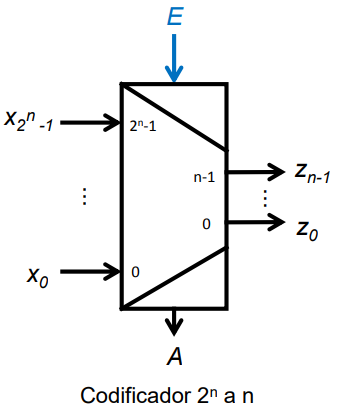
\includegraphics[scale=0.65]{codificador}
\end{center}

\begin{center}
\begin{tabular}{|c|c|c|c|c|c|c|c|}
\hline
$E$ & $x_0$ & $x_1$ & $x_2$ & $x_3$& $z_0$ & $z_1$ & $A$ \\
\hline
0 & - & - & - & - & 0 & 0 & 0 \\
\hline
1 & 0 & 0 & 0 & 0 & 0 & 0 & 0 \\
\hline
1 & 0 & 0 & 0 & 1 & 0 & 0 & 1 \\
\hline
1 & 0 & 0 & 1 & 0 & 0 & 1 & 1 \\
\hline
1 & 0 & 1 & 0 & 0 & 1 & 0 & 1 \\
\hline
1 & 1 & 0 & 0 & 0 & 1 & 1 & 1 \\
\hline
\end{tabular}
\end{center}
\end{multicols}

Es decir, la salida codifica en binario el valor del subíncide de la entrada activada. La función de la salida de actividad es distinguir cual de los 3 casos en los que salida es 0 es el válido y real para las entradas que hay en ese momento, es decir, cuando la única variable activa es $x_0$ y el enable $E=1$, entonces $A=1$.

\begin{center}
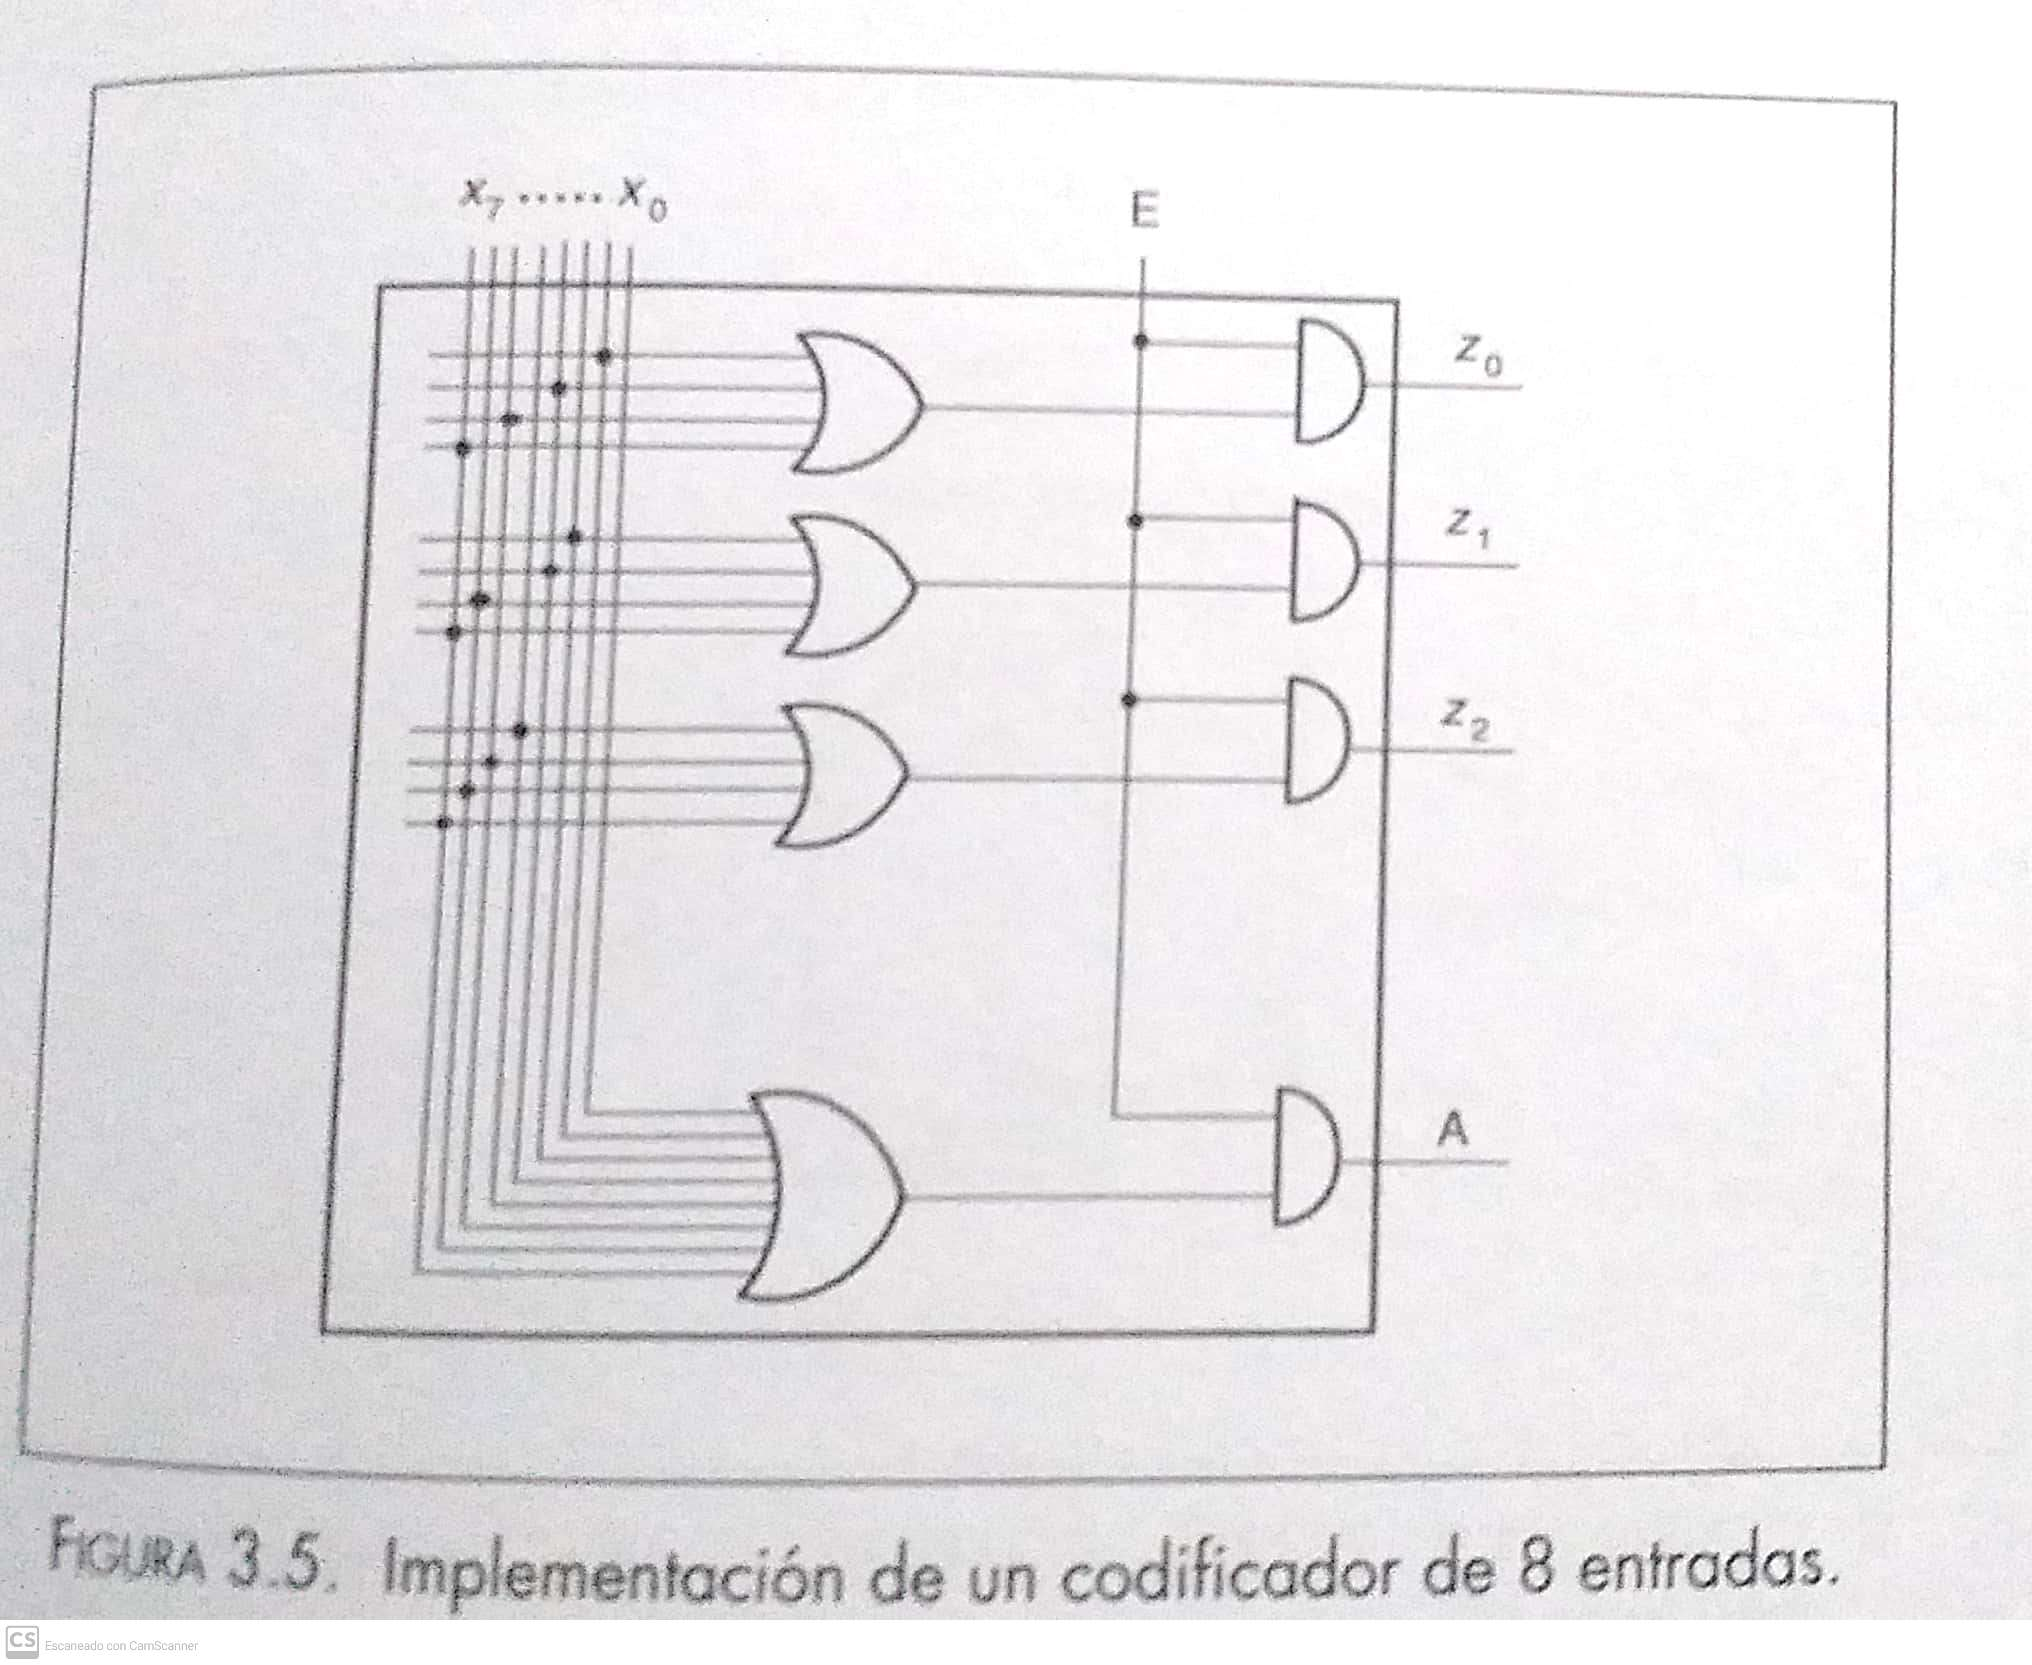
\includegraphics[scale=0.12]{codificador tripas}
\end{center}

Este es un ejemplo de la implementación directa de un codificador de 8 a 3. Se puede observar que la salida $A$ solo vale 1 cuando alguna de las entradas está activa y que las salidas $z_i$ solo pueden valer 1 si el \textit{enable} se lo permite. De este modo cada puerta \textit{OR} da valor 1 a la salida correspondiente cuando algunas de las entradas $x_i$ con las que se activa, está activa.

\subsubsection*{Codificador de prioridad}
Se ve de la definición prestada antes que el caso en el que más de una entrada está activa supone un problema de indeterminación en el diseño, para evadir dicho vacío lógico sirve el \textbf{codificador de prioridad} cuya función es establecer prioridades entre las diferentes entradas del mismo.

\begin{center}
\includegraphics[scale=0.23]{codificador de prioridad}
\end{center}

Podemos observar que lo único necesario para poder implementar este tipo de codificador es un módulo anterior que resuelva las prioridades y le pase a un codificador usual las entradas correspondientes de la forma en que se ha explicado en el apartado anterior (todo 0 menos alguna en 1).\par

Podemos ver en esta nueva definición una nueva salida, $E_{out}$ o \textit{salida de capacitación} que, como vemos, solo vale 1 si la entrada de capacitación es 1, es decir, está habilitado, pero la salida de actividad vale 0, es decir, no está en funcionamiento, a pesar de que está habilitado. La función de esta nueva salida no es más que posibilitar la combinación de varios de estos módulos para obtener uno igual pero con mayor número de entradas.

\begin{center}
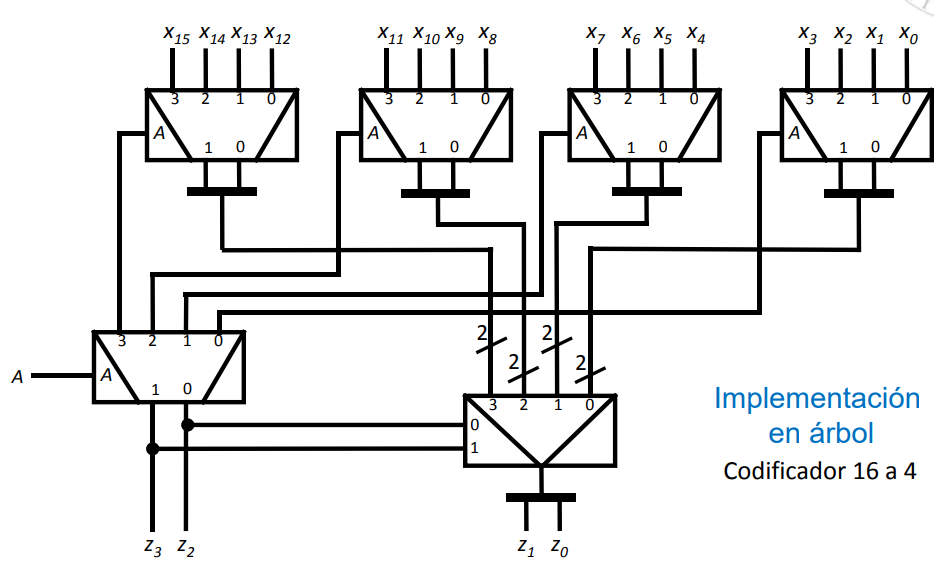
\includegraphics[scale=0.50]{combinacion de codificadores1}
\end{center}

\begin{center}
\includegraphics[scale=0.50]{combinación de codificadores2}
\end{center}

La implementación directa del resolutor de prioridades comentado anteriormente quedaría de la siguiente forma\footnote{Se puede apreciar por las características de su diseño que este es fácilmente escalable al número de entradas deseado por lo que no supone mayor complicación fabricar uno más grande}:

\begin{center}
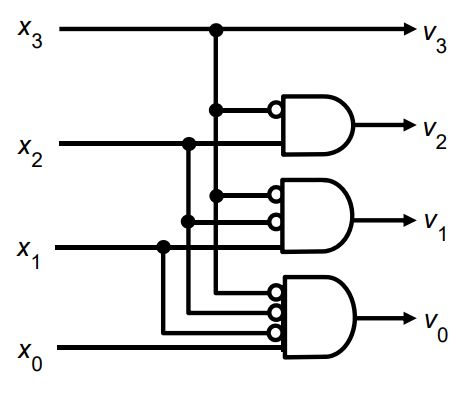
\includegraphics[scale=0.60]{resolutor de prioridades tripas}
\end{center}

\subsubsection*{Aplicaciones de diseño}
Una de las posibles aplicaciones es la asociación de un código a cada componente de un vector de entrada. Supongamos que tenemos un teclado con 30 teclas, entonces serían necesarias $2^5$ entradas en un decodificador y cada tecla pondría a 1 su $x_i$ correspondiente, esto haría que cada tecla tuviera asociado un vector en binario de salida que identificaría dicha tecla.

\begin{center}
\includegraphics[scale=0.53]{aplicacion de diseño codificador}
\end{center}


\subsection*{\underline{Multiplexor}}
Es un módulo combinacional que redirige el flujo de entrada desde una de las entradas a una de las salidas y posee las siguientes partes:
\begin{itemize}
\item $2^n$ entradas binarias ($x_i$)
\item $n$ entradas de control (s)
\item Una única salida (z)
\item Puede tener un enable (E)
\end{itemize}
$z=a_i$ donde i es la el valor en decimal de la codificación del número de n bits de la entrada de control (s):
$$z=E\cdot \sum (x_i\cdot m_i(s))$$

\begin{multicols}{2}

\begin{center}
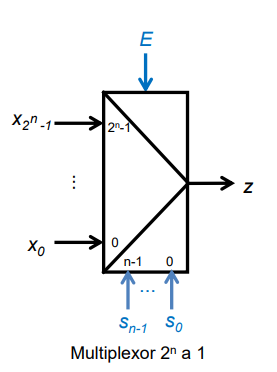
\includegraphics[scale=0.80]{multiplexor}
\end{center}

\begin{center}
\begin{tabular}{|c|c|c|c|}
\hline
$s$ & $x_0$ & $x_1$ & z \\
\hline
0 & 0 & 0 & 0 \\
\hline
0 & 0 & 1 & 0 \\
\hline
0 & 1 & 0 & 1 \\
\hline
0 & 1 & 1 & 1 \\
\hline
1 & 0 & 0 & 0 \\
\hline
1 & 0 & 1 & 1 \\
\hline
1 & 1 & 0 & 0 \\
\hline
1 & 1 & 1 & 1 \\
\hline
\end{tabular}
\end{center}
\end{multicols}
Se observa que cuando la entrada de control vale 1, la salida  $z$ toma el valor que tuviese en ese momento la entrada $x_1$ y cuando vale 0, el valor de $x_0$.\par
La implementación del circuito interno quedaría de la siguiente forma:
\begin{center}
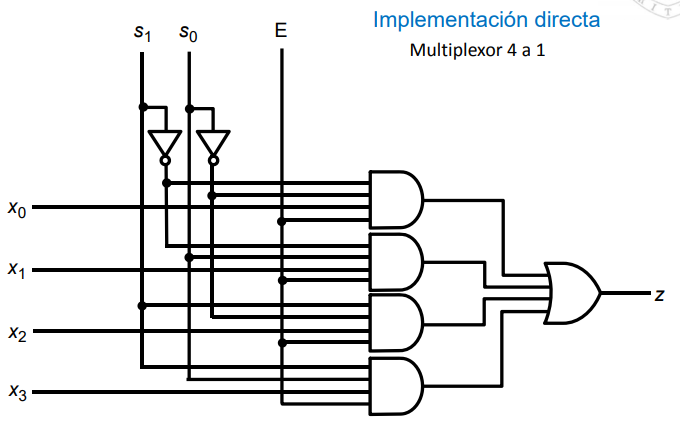
\includegraphics[scale=0.75]{implementacion multiplexor}
\end{center}

Es fácil ver que la implementación interna del funcionamiento de este dispositivo tiene mucho que ver con la del decodificador, hasta tal punto que la única diferencia entre ambos es la inclusión de una puerta \textit{OR} en el multiplexor por lo que la implementación de este módulo también puede hacerse a partir de un decodificador cuyas salidas están conectadas a una puerta \textit{OR} que define la función del multiplexor en contra posición a la del decodificador.\par

La implementación de un multiplexor de más entradas es posible a través de la combinación de otros más pequeños. El procedimiento más habitual el siguiente:
\begin{center}
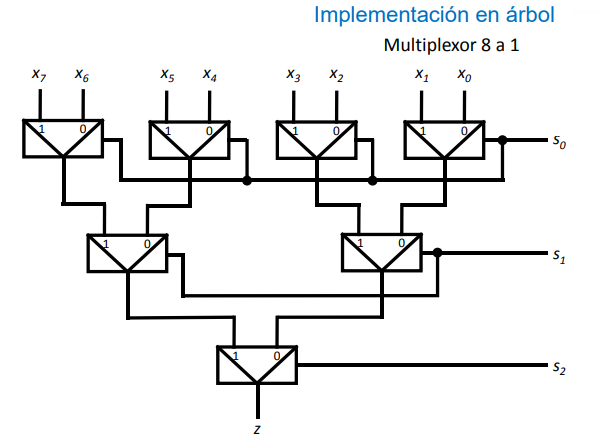
\includegraphics[scale=0.75]{arbol multiplexor}
\end{center}

\subsubsection*{Aplicaciones de diseño}
Es razonable pensar que si un decodificador junto con varias puertas \textit{OR} era capaz de implementar cualquier función de conmutación como suma de productos canónica, como el multiplexor lleva ya implementada dicha puerta, entonces un multiplexor es capaz de implementar cualquier FC. Y en efecto, el multiplexor es un \textbf{conjunto universal} de los estudiados anteriormente, aunque el diseño con el uso exclusivo de los mismo puede no ser siempre demasiado intuitivo, pero sí posible.\par

Un procedimiento general para implementar cualquier función de $n$ variables es el siguiente:
\begin{itemize}
\item El vector de entradas de control será el vector formado por las variables de la FC.

\item En el vector de entradas de datos, cada $x_i$ será el valor de cada minterm de la FC \textbf{en orden}, es decir, cada $x_i$ será el valor de la función en ese punto del dominio.

\begin{center}
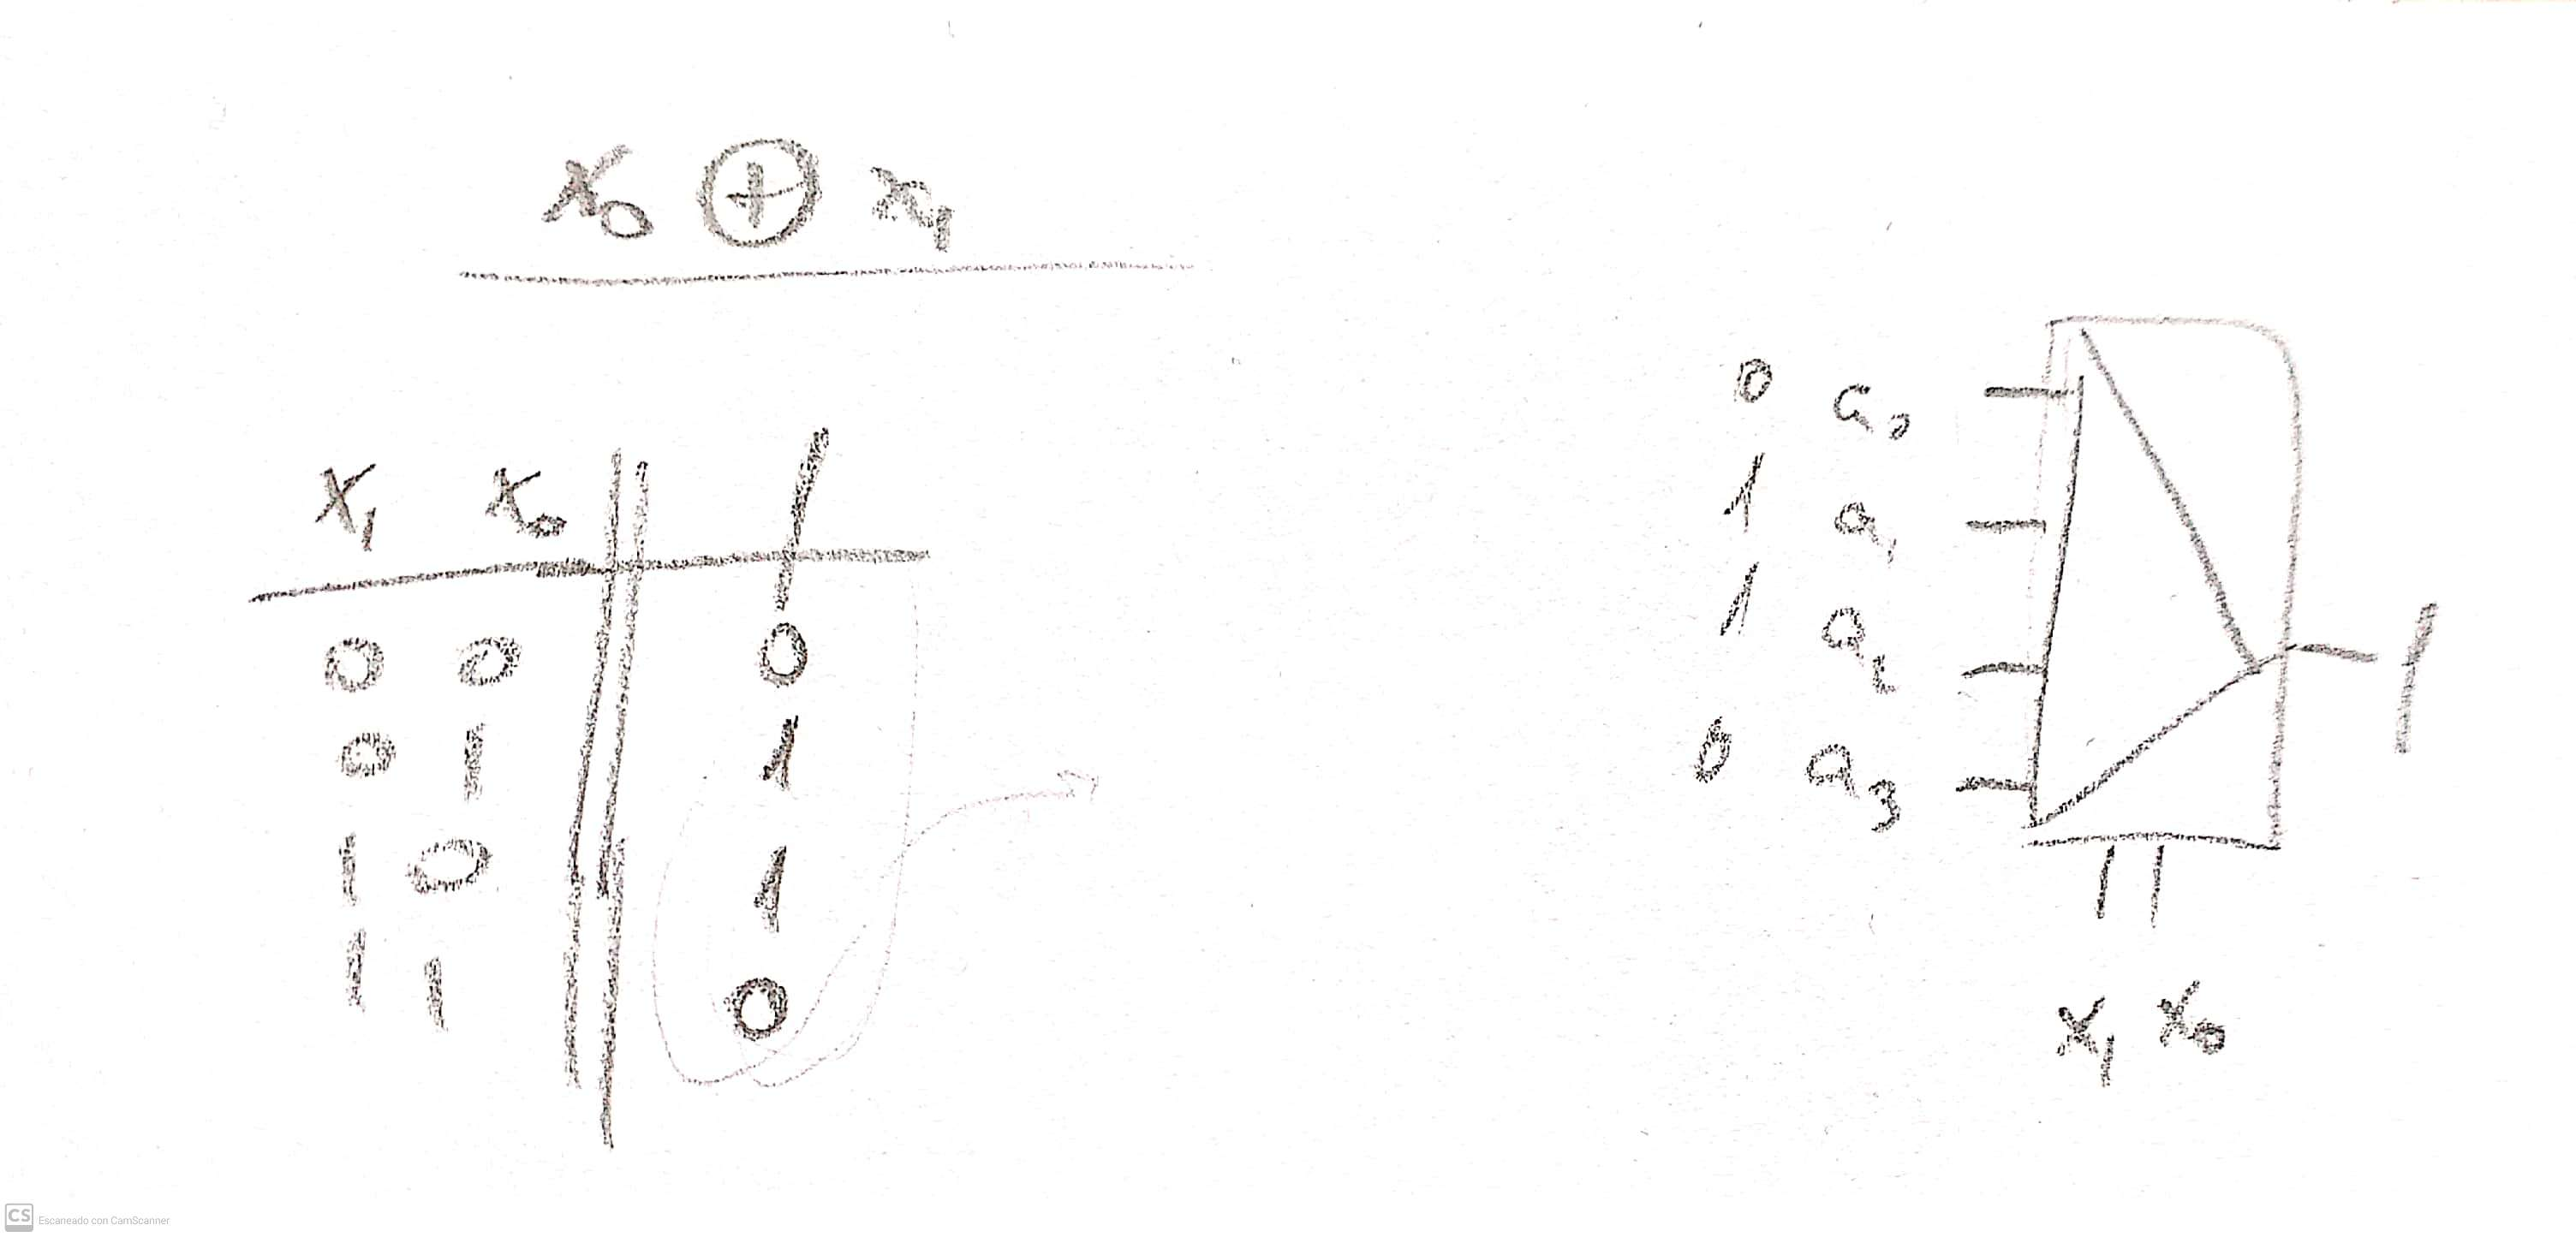
\includegraphics[scale=0.08]{aplicacion multiplexor 1}
\end{center}
\end{itemize}

Cuando tenemos que implementar una función de $n+k$ variables y tenemos solo disponible un multiplexor de $n$ entradas de control el procedimiento es:
\begin{itemize}
\item Elegimos $n$ variables que serán nuestras entradas de control.

\item De la suma de productos canónica, extraemos factor común de esas variables en todas las combinaciones posibles y simplificamos el resultado.

\item Cada paréntesis resultante es una función de conmutación auxiliar que va a cada entrada de datos del multiplexor.

\begin{center}
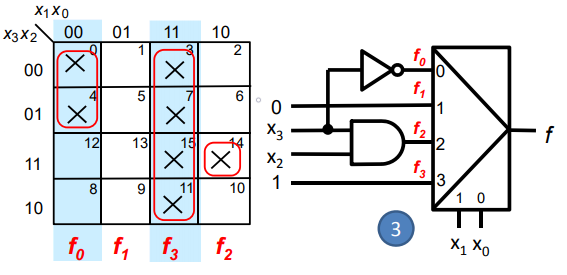
\includegraphics[scale=0.50]{aplicacion multiplexor 2}
\end{center}

Conviene saber que la elección de las variables de control determina si una implementación es más eficiente que otra o la forma de escoger las $f$ auxiliares porque, una vez hechos los grupos de karnaugh según las reglas ya explicadas no podemos separar a miembros del mismo grupo y como se ve en el siguiente ejemplo, el considerar que cada $f$ es una fila porque son $x_0$ y $x_1$ las que son variables de control ya no es posible y hay que elegir otras.

\begin{center}
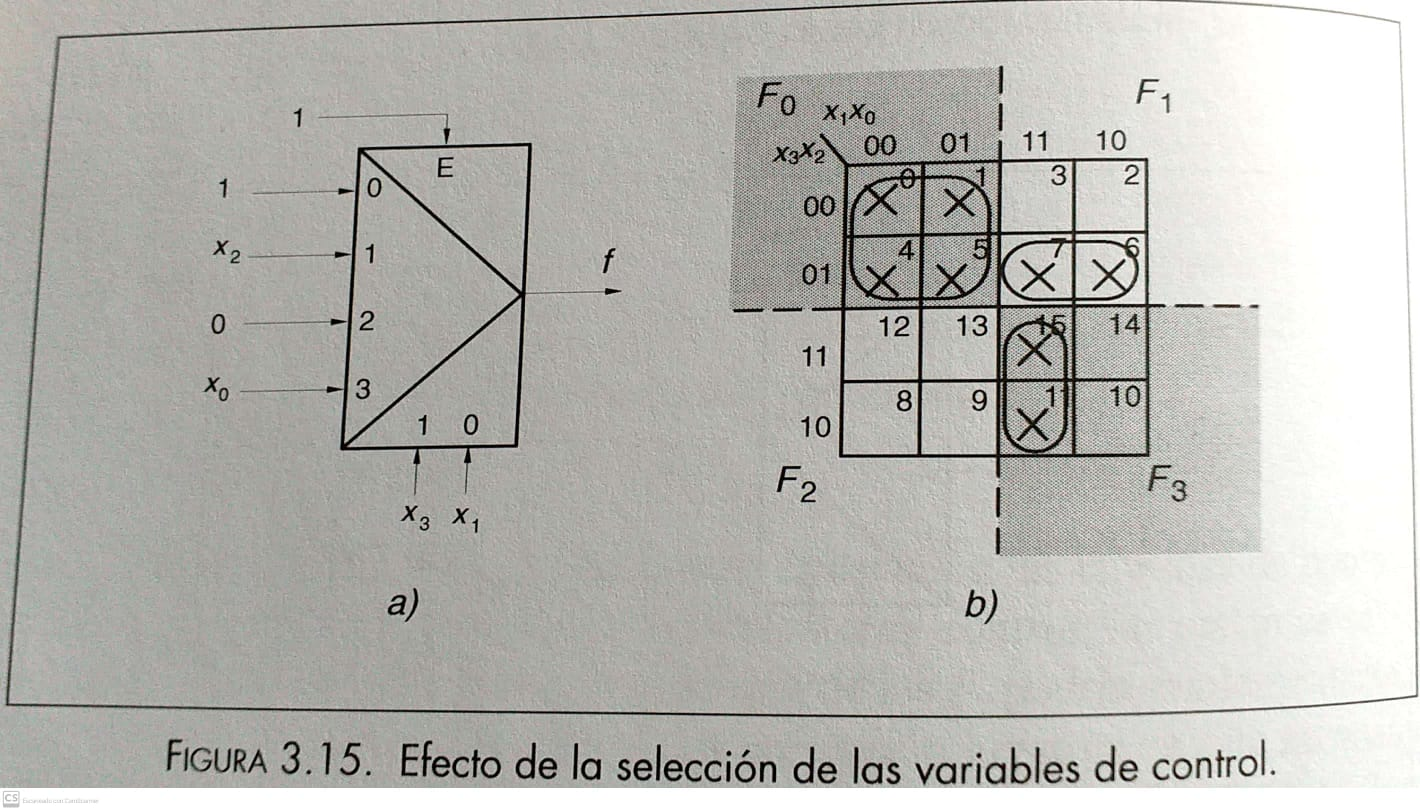
\includegraphics[scale=0.17]{aplicacion multiplexor 3}
\end{center}

\end{itemize}

\subsection*{\underline{Sumador/Restador}}
\subsubsection*{Sumador}
Las entradas son 3, dos bits que hay que sumar y un bit que determina si esa operación tiene un acarreo de otra anterior o no (porque se suelen usar combinados), las salidas son 2, una que determina el resultado de la suma de los dos bits de entrada y otra que le añade a la salida un un bit si hubiese acarreo.

\begin{multicols}{2}
	
\begin{center}
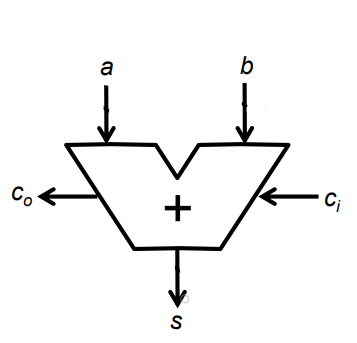
\includegraphics[scale=0.45]{sumador simple}
\end{center}

\begin{center}
\begin{tabular}{|c|c|c|c|c|}
\hline
$c_i$ & a & b & $c_0$ & s \\
\hline
0 & 0 & 0 & 0 & 0 \\
\hline
0 & 0 & 1 & 0 & 1 \\
\hline
0 & 1 & 0 & 0 & 1 \\
\hline
0 & 1 & 1 & 1 & 0 \\
\hline
1 & 0 & 0 & 0 & 1 \\
\hline
1 & 0 & 1 & 1 & 0 \\
\hline
1 & 1 & 0 & 1 & 0 \\
\hline
1 & 1 & 1 & 1 & 1 \\
\hline
\end{tabular}
\end{center}

\end{multicols}

El funcionamiento es similar para un sumador más de 2 bits. Se colocan en serie varios sumadores simples de modo que el acarreo de salida de uno sea el de entrada del siguiente así que realizan el proceso de sumar a mano que conocemos de toda la vida, el aspecto de la combinación de varios para sumar vectores binarios es:

\begin{center}
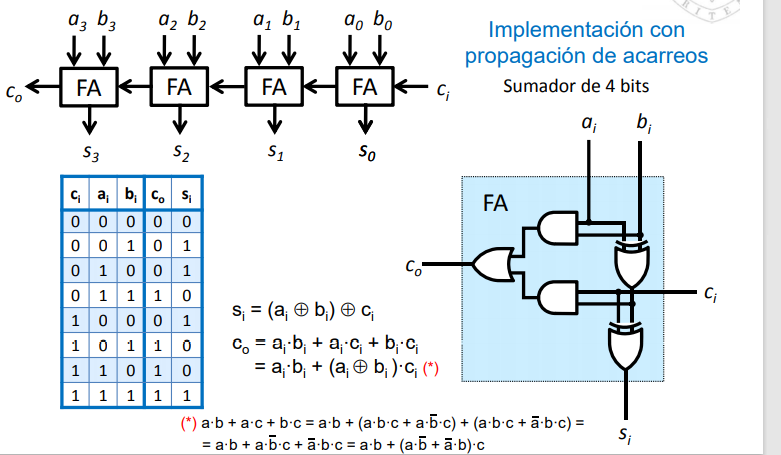
\includegraphics[scale=0.55]{sumador en serie}
\end{center}

Este sumador sumaría dos número de 4 bits cada uno.

\subsubsection*{Restador}
Los ordenadores en general suele funcionar en $C_2$, para ello la operación de resta se puede expresar como:
$$A-B=A+B_{C_2}=A+(B_{C_1}+1)=A+\bar{B}+1$$
Quedando el sumador resultante como:

\begin{multicols}{2}
\begin{center}
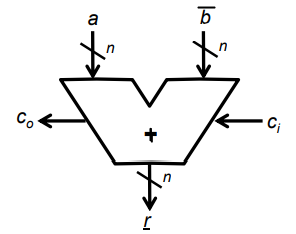
\includegraphics[scale=0.55]{restador sencillo}
\end{center}

\begin{center}
\begin{tabular}{|c|c|c|c|c|c|c|c|c|c|c|}
\hline
$c_i$ & $a_2$ & $a_1$ & $a_0$ & $b_2$ & $b_1$ & $b_0$ & $c_0$ & $r_2$ & $r_1$ & $r_0$ \\
\hline
0 & 0 & 1 & 1 & 0 & 1 & 0 & 0 & 0 & 1 & 0\\
\hline
\end{tabular}
\end{center}
\end{multicols}

De este modo, el restador no es más que un sumador de opuestos 1. Del mismo modo, varios se pueden componer en serie para conseguir uno de mayor anchura.

\begin{center}
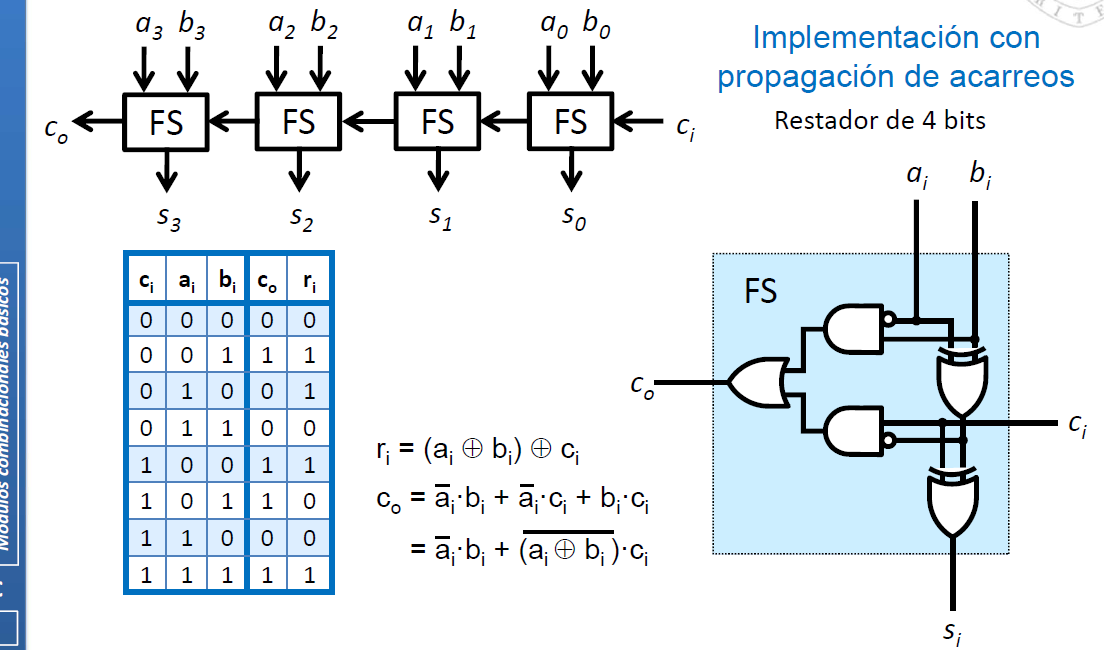
\includegraphics[scale=0.5]{Restador tripas}
\end{center}

\subsubsection*{Sumador/Restador}
Para no tener que distinguir entre ambos módulos y al observar que en esencia ambos son sumadores (aunque uno de ellos sume el opuesto), podemos implementar uno único módulo que realice la función de ambos y que pueda seleccionar que operación hacer.

\begin{center}
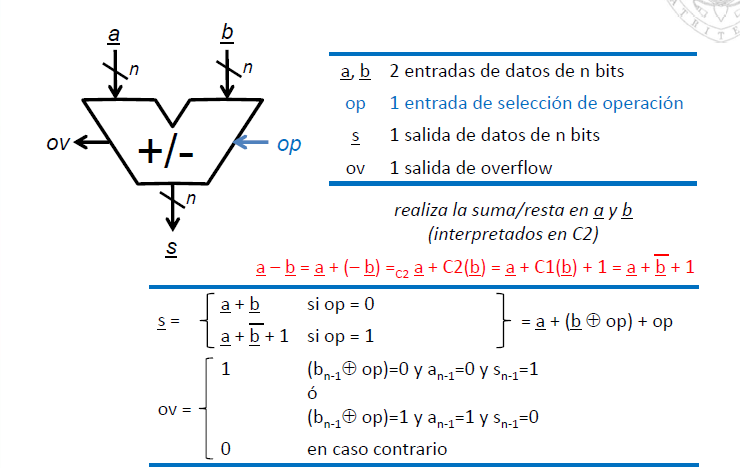
\includegraphics[scale=0.75]{sumador_restador}
\end{center}

\begin{center}
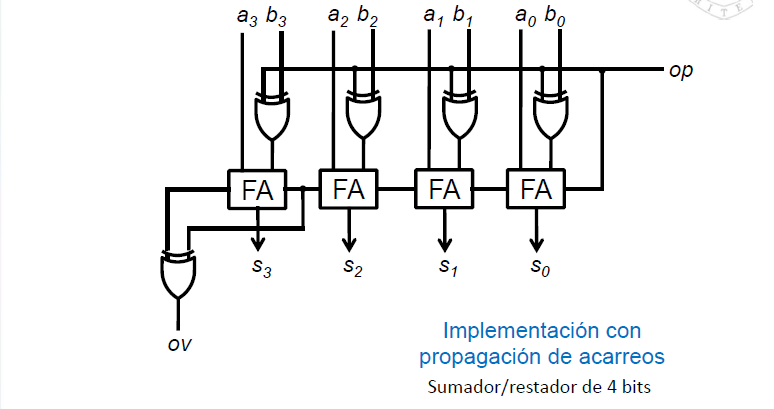
\includegraphics[scale=0.75]{sumador_restador_tripas}
\end{center}

\subsection*{\underline{ALU}}
Esta unidad realiza las operaciones aritmético-lógicas básicas de un microprocesador. Este módulo posee:
\begin{itemize}
\item 2 entradas de datos de \textit{n} bits
\item 1 entrada de selección de modo (aritmético o lógico)
\item 1 entrada de selección de operación\footnote{Será de un número \textit{n} de bits en función del número de operaciones que soporte}
\item 1 salida de datos de \textit{n} bits
\item 4 salidas de control de datos como se especifica en la imagen
\end{itemize}

\begin{center}
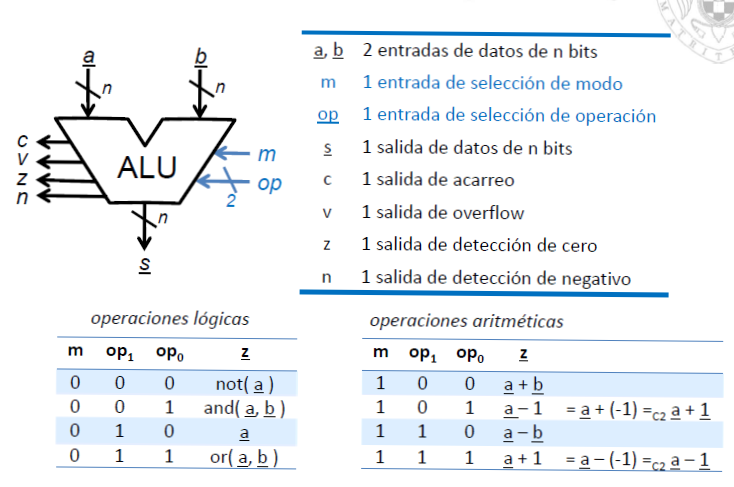
\includegraphics[scale=0.75]{ALU_diseño}
\end{center}

El funcionamiento interno se puede interpretar de distintas formas:

\subsubsection*{Módulos separados}

\begin{center}
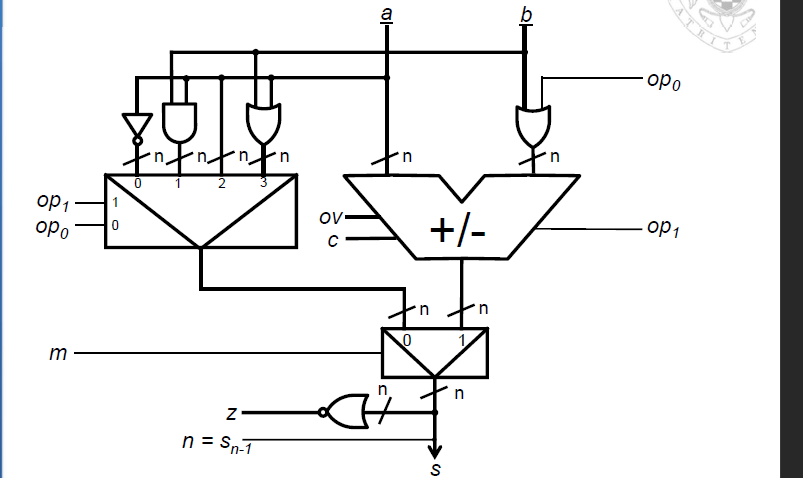
\includegraphics[scale=0.74]{ALU1}
\end{center}

De esta forma vemos que la parte del sumador de la derecha corresponde a las operaciones aritméticas y la parte del multiplexor de la izquierda corresponde a las operaciones lógicas. Las entradas de selección \textit{op} determinan el tipo de operación que realiza cada una de las dos partes y finalmente la entrada \textit{m} determina cuál de las dos operaciones, la aritmética o la lógica, se muestran finalmente. Es decir, en este caso se evalúan ambas formas y al final es cuando se decide cuál mostrar.

\subsubsection*{Módulos adicionales a un sumador total}
En este caso, lo que se hace es añadir dos módulos conocidos como ampliadores lógicos \textit{(LE)} y aritméticos \textit{(AE)} a un sumador total. De esta forma, si se emplea la función aritmética, ya hemos estudiado como debería funcionar un sumador/restador, pero si se emplea la función lógica, entonces los sumadores no son más que meras conexiones de retardo fijo, es decir, no suman nada.

\begin{center}
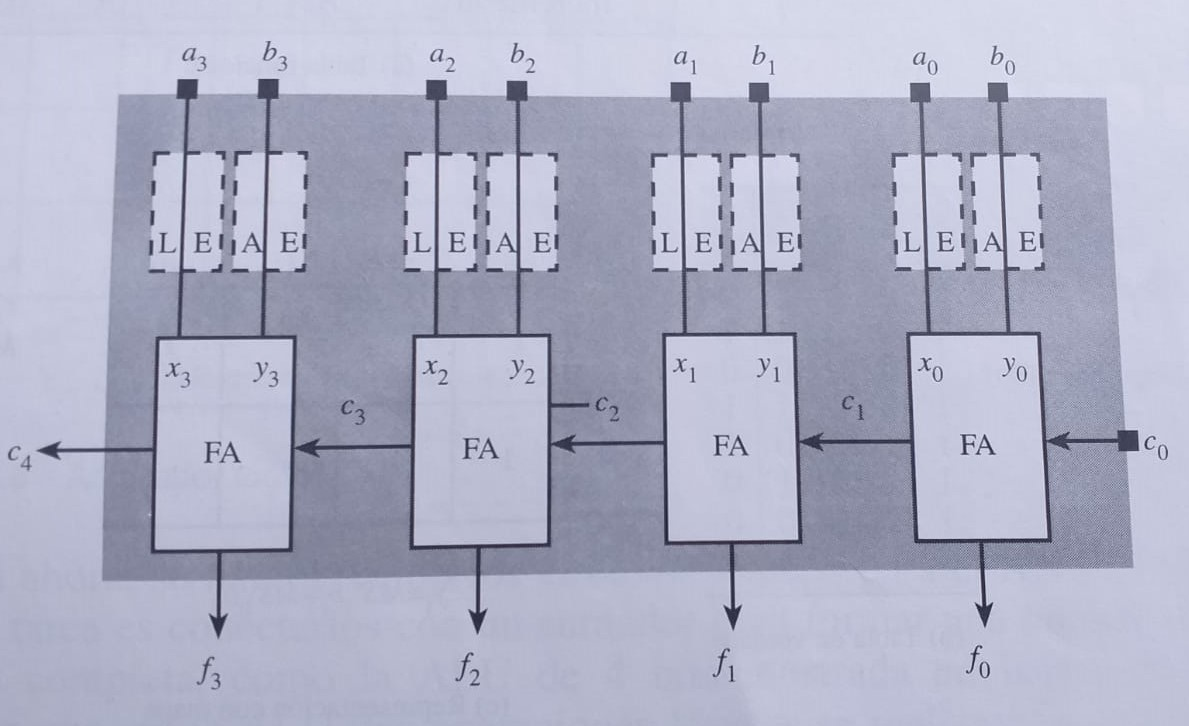
\includegraphics[scale=0.37]{ALU2}
\end{center}

Podemos ver en la tabla de verdad de abajo que el funcionamiento descrito en el módulo \textit{AE} es completamente anágolo a como funcionaría en el ejemplo anterior, siendo la foto de abajo el funcionamiento de cada uno para un bit concreto.

\begin{center}
\includegraphics[scale=0.37]{Ampliador_aritmetico}
\end{center}

Para la parte lógico podemos observar que la parte de \textit{Y} es siempre 0 en la tabla de verdad. Esta es la diferencia fundamental con respecto al ejemplo anterior de tipo de ALU puesto que en este caso \textbf{toda la condición se pasa como vector a las entradas \textit{a}}. Con lo cual, es fácil ver que en este caso el sumador no suma nada, porque suma 0 con algo, y que en consecuencia la salida es directamente la condición evaluada.

\begin{center}
\includegraphics[scale=0.35]{Ampliador_logico}
\end{center}

La ALU resultante según este tipo quedaría de la siguiente forma:
\begin{center}
\includegraphics[scale=0.37]{ALU_final}
\end{center}

\subsection*{\underline{ROM}}
La ROM (\textit{Read Only Memory}) es un módulo combinacional formado por los siguientes elementos:
\begin{itemize}
\item Entradas de dirección (x)
\item Salidas de datos (z)
\item Entrada de capacitación (CE)
\item Entrada de capacitación de lectura (OE)
\end{itemize}
La entrada de capacitación es su \textit{enable} personal y determina el funcionamiento o no del módulo, la entrada de capacitación de lectura	es necesaria para implementar ROMs de más tamaño y sirve para pasar un valor que hará de enable en el resto de ROM que formen una más grande.

\begin{multicols}{2}
\begin{center}
\includegraphics[scale=0.65]{ROM}
\end{center}

\begin{center}
\includegraphics[scale=0.35]{matrices ROM}
\end{center}
\end{multicols}


A diferencia de los módulos anteriores, este módulo no posee una fórmula específica para la descripción de los valores de salida. Se trata de un dispositivo que al igual que el decodificador, implementa todos los minterms en la matriz AND y a cada uno le asigna una dirección de entrada, posteriormente y en función de la configuración interna, devuelve los valores que están guardados en cada dirección, por este motivo decimos que es una memoria, porque en el fondo guardamos en cada dirección un array de bits que posteriormente se reproducen en las salidas de datos al haber introducido una dirección dada.

\begin{center}
\includegraphics[scale=0.65]{ROM 3}
\end{center}

Es decir, observamos, sobre todo tras hacer la representación con un decodificador\footnote{Por cuestión de claridad, al haber muchas entradas para cada puerta \textit{OR} el dibujo puede complicarse así que en vez de poner todas las líneas se pon una única que representa a todas y se marcan en los que puede valer 1}, que las entradas $a$ indican el minterm o dirección en el cuál mirar y las salidas $d$ devuelven los valores de ese minterm para cada salida de la FC o podemos llamarlos los ``datos'' guardados en esa dirección.

Tenemos también varias modificaciones del concepto de ROM para atribuirle distintas funcionalidades:

\begin{itemize}
\item \textbf{Mask Programmable ROM}
	\begin{itemize}
	\item Se programa durante la fabricación del chip.
	\item No puede borrarse/reprogramarse.
	\end{itemize}
\item \textbf{PROM (Programmable ROM)}
	\begin{itemize}
	\item Se programa eléctricamente usando un programador.
	\item No puede borrarse/reprogramarse.
	\end{itemize}
\item \textbf{EPROM (Erasable Programmable ROM)}
	\begin{itemize}
	\item Se programa eléctricamente usando un progamador.
	\item Se borra (chip completo) exponiéndola a luz ultravioleta.
	\end{itemize}
\item \textbf{EEPROM (Electrically Erasable Programmable ROM)}
	\begin{itemize}
	\item Se programa/borra (palabra) eléctricamente usando un programador.
	\end{itemize}
\item \textbf{Flash memory}
	\begin{itemize}
	\item Se programa/borra (bloque) eléctricamente sin requerir programador.
	\end{itemize}
\end{itemize}

\subsubsection*{Aplicaciones de Diseño}
A parte de que podemos implementar (según la imagen introducida más arriba) $n$ FC de $k$ variables cada una, podemos combinar varias de ellas para conseguir dos funcionalidades:
\begin{itemize}
\item \textbf{Anchura de palabra}:\par
	Esto nos permite tener más valores guardados en cada dirección para el mismo número de direcciones.

\begin{center}
\includegraphics[scale=0.60]{ROM anchura palabra}
\end{center}

Es decir, para crear dicha combinación de módulos lo que hacemos es que las entradas de dirección se pasan a todas las ROM, el enable de la 1ª se pasa a las demás y las salidas de cada una se juntan todas en un único vector de salida ORDENADO que se hace usando el BUS de abajo.

\item \textbf{Profundidad}:\par
Esto nos permite tener más direcciones posibles pero con el mismo número de valores que se pueden guardar en cada una.

\begin{center}
\includegraphics[scale=0.55]{ROM profundidad}
\end{center}

En el fondo es más útil pensarlo conmo si se dispusiesen en vertical para ver que son más entradas de dirección y la misma longitud de palabra. El decodificador hace que se distingan las ROM que hay que utilizar en función de los dos valores de más peso siendo las direcciones que comienzan por $00$ las de la primera ROM y $11$ las de la última. Cuando la combinación de los valores más significativos es ese, la entrada de capacitación de lectura se habilita SOLO EN UNA DE LAS ROM y por lo tanto hemos indicado que solo vamos a buscar en ese módulo. Lo demás es igual que la ROM aislada, una vez que tenemos seleccionada cuál debe funcionar, el resto del nombre de la dirección se busca en la ROM y como las OE del resto de ROMs están desactivadas no hay ningún problema con respecto a cortocircuitar las salidas con el BUS de la imagen puesto que solo hay corriente por las salidas de datos de la ROM en la que buscábamos y de este modo se devuelven los valores guardados en la dirección deseada.

\end{itemize}

\subsection*{\underline{Comparador de magnitud}}
Se usa para evaluar los operadores lógicos $<$, $=$ y $>$. Para ello este módulo se compone de las siguientes partes:
\begin{itemize}
\item 2 entradas de \textit{n} datos
\item 2 entradas de acarreo
\item 2 salidas de comparación
\end{itemize}

\begin{center}
\includegraphics[scale=0.65]{comparador_magnitud}
\end{center}

\begin{center}
\includegraphics[scale=0.69]{comparador1}
\end{center}

Los valores de salidas dependen de dos posibilidades, valdrán 1 automáticamente si un bit es menor que el otro o viceversa o también valdrán 1 en caso de que siendo iguales las entradas de acarreo reflejen que los de antes no lo eran. Viendo este funcionamiento en función de los valores anteriores, podemos ver de forma intuitiva que si se combinan de la misma forma que lo hacían los sumadores podemos componer comparadores de palabras de más bits.
\begin{center}
\includegraphics[scale=0.64]{comparador2}
\end{center}

Lo que podemos ver en el funcionamiento interno es que la comparación de dos números enteros positivos\footnote{Nótese que dicha descripción es sólo válida para números positivos} se reduce a la comparación exclusiva de dos bits, comenzando por los menos significativos y yendo hacia los que más.

\subsection*{\underline{Aspectos tecnológicos}}
Para calcular el gasto de los módulos combinacionales en lo que a retardo, precio y área se refiere, procedemos de forma igual que en las redes de puertas, pero en este caso con la correspondiente tabla:

\begin{center}
\includegraphics[scale=0.64]{gasto modulos}
\end{center}

\chapter*{ESPECIFICACIÓN DE SISTEMAS SECUENCIALES}
\section*{ESPECIFICACIÓN DE ALTO NIVEL}
La diferencia fundamental que presenta este tipo de sistemas con respecto a los combinacionales es que si para estos últimos una misma entrada tenía un única posible salida, para los secuenciales una misma entrada puede tener distintas salidas en función de cual sea la secuencia de entradas anteriores. Es decir, si para la entrada 1, la salida vale 0, en los sistemas secuenciales la salida puede pasar a valer 1 pasado un cierto tiempo cuando en los sistemas combinacionales la salida se mantiene invariante.

Veamos un ejemplo:\par
\textit{Supongamos que tenemos una máquina que indica si el número de 1 que ha recibido a lo largo del tiempo es par o impar}.
$$\begin{array}{cccccc}
A = & 0 & 0 & 1 & 0 & 1 \\
B = & 1 & 0 & 1 & 1 & 0 \\
C = & 0 & 1 & 1 & 0 & 1 \\
D = & 1 & 1 & 1 & 0 & 1   
\end{array}$$

Observamos claramente que para ambas secuencias de entradas $A$ y $D$ tenemos que la salida deberá indicar el mismo valor, al igual que ocurre con las secuencias $B$ y $C$ entre ellas. De este modo, vemos que el sistema en el caso de la secuencia $A$ o $D$ solo puede variar de una forma concreta:
$$\begin{cases}x(t)=0 & \rightarrow z(t)=1 \\ x(t)=1 & \rightarrow z(t)=0
\end{cases}$$

Es decir, decimos que si la secuencia que tenemos es de un número de 1 PAR, entonces si recibe otro 1 cambiará a una de tipo PAR y la salida valdrá 0 y si recibe un 0 seguirá siendo PAR y la salida seguirá siendo 1.\par

Es evidente que cualquier secuencia de entrada se puede agrupar en dos clases distintas, una secuencia con un número par de 1 o con un número impar. De esta dicotomía surge el concepto denomidado \textbf{ESTADO}, que no es más que el conjunto de las secuencias que causan el mismo efecto y que determina la situación del sistema en función de la secuencia de entradas previas. De esto modo, conociendo el estado en el que me encuentro soy capaz de determinar en función de mi entrada, cual será mi salida y mi estado futuros.

Una vez visto el concepto de sistema secuencial y las peculiaridades que presenta es notable resaltar que hay dos posibles formas de afrontar la especificación de estos sistemas. Podemos hacer que \textbf{la salida dependa directamente del estado en el que me encuentro} o que \textbf{la salida dependa del estado y entrada anteriores}. De estos dos enfoques nacen las \textbf{máquinas de Mealy y de Moore}.

\subsection*{\underline{Máquinas de Mealy y de Moore}}

Es notable destacar antes de entrar en la descripción de ambos modelos que cualquier sistema secuencial se puede especificar de cualquiera de las dos formas y que la existencia de ambas es para la optimización de los diseños creados, cuya evaluación se deja a cuenta del diseñador.
\subsubsection*{Máquinas Mealy}
Las máquinas de Mealy se decantan por la opción 2, es decir, en este tipo de sistemas secuenciales la salida es una función de la entrada y estado actuales, con lo cual siempre la salida refleja el valor en función de la entrada actual y \textbf{NO va con retraso}.
$$\begin{cases} z(t)=H(x(t),s(t)) & \mbox{ donde H es la función que define la salida} \\ s(t+1)=G(s(t),x(t)) & \mbox{ donde }G\mbox{ es la función que define el estado}\end{cases}$$

Para la descripción de estas máquinas es útil utilizar los conocidos como \textbf{diagramas de estados}:
\begin{center}
\includegraphics[scale=0.45]{diagrama1}
\end{center}

En este tipo de diagramas se indican los cambios con la siguiente notación:
\begin{itemize}
\item Cada estado se escribe dentro de un círculo
\item Se trazan tantas flechas como posibles entradas haya
\item Cada flecha se dirige al siguiente estado según la entrada recibida
\item En cada flecha se escribe de numerador la entrada que provoca el cambio y de denominador la salida que refleja
\end{itemize}

Ej.:
\begin{center}
\includegraphics[scale=0.30]{ejemplo_diagrama1}
\end{center}

\subsubsection*{Máquinas de Moore}
Las máquinas de Moore se decantan por la opción 1; la salida depende exclusivamente del estado actual. Con lo cual, las funciones que definen el estado y la salida en un ciclo de reloj $t$ nos quedan como:
$$\begin{cases} z(t)=H(s(t)) & \mbox{ donde H es la función que define la salida} \\ s(t+1)=G(s(t),x(t)) & \mbox{ donde }G\mbox{ es la función que define el estado}\end{cases}$$

Con lo cual, podemos ver que la salida que vemos en un instante $t$ es consecuencia de la entrada del instante $t-1$, por lo que nuestro sistema da salidas con un retraso de un ciclo de reloj\footnote{Lo cual es muy significativo al combinar estas máquinas con otras que sean síncronas} con respecto a las máquinas de Mealy.

En este caso la representación mediante diagramas de cambio de estado también es útil, eso sí, cambiando debidamente la notación correspondiente:
\begin{itemize}
\item Se escribe la salida como denomidador del estado dentro del círculo, pues depende del mismo.
\item Las flechas siguen el mismo funcionamiento pero ahora solo se indica la entrada que provoca el cambio de estado.
\end{itemize}
\begin{center}
\includegraphics[scale=0.35]{ejemplo_diagrama2}
\end{center}

\subsubsection*{Simplificación de estados}
En general, puede ocurrir que al definir el comportamiento de un sistema secuencial, tengamos en cuenta más estados de los que realmente son necesarios, lo que encarece el circuito y contribuye al retardo de las señales.
Aunque existen procedimiento sofisticados de computación para poder hacer esto, una forma más sencilla pero prácticamente igual de efectiva es tener en cuenta la siguiente norma, sean $s_1$ y $s_2$ dos estados del sistema:
$$s_1\equiv s_2 \Leftrightarrow H(s_1, x)=H(s_2, x)$$
$$s_1\equiv s_2 \Leftrightarrow G(s_1, x)=G(s_2, x)$$

Es decir, dos estados \textbf{son equivalentes} si poseen la misma salida para la misma combinación de entrada y confluyen al mismo siguiente estado para la misma combinacion de entrada. Si se dan estas dos condiciones, entonces podemos escribir dicho estado como el mismo, simplificando la síntesis de nuestro sistema secuencial.

\subsection*{\underline{Especificación binaria}}
Para la codificación binaria de estos sistemas no hay más que escribir las tablas de verdad que hacíamos en temas anteriores para cada función de conmutación y tras haberlo definido todo, dar una codificación binaria a cada valor posible.
El cálculo del resto de cosas, como la simplificación de las FC, los retardos, etc. es análogo a lo anterior y si cupiese alguna duda se recomienda mirar capítulos anteriores, el ejemplo del tema posterior de implementación o el propio libro de Fundamentos de Commputadores que se posea.

\subsubsection*{Codificación eficiente}
Como se verá posteriormente, una codificación u otra de las entradas, salidas, estados... repercutirá en el número de puertas, biestables, entradas... y, por lo tanto, en el diseño, su gasto y su retardo. Por ello, es primordial tener en cuenta algún método que permita tener una implementación óptima en cuanto a la codificación se refiere, para ello, basta con seguir estas reglas:
\begin{itemize}
\item Hacer el diagrama de estados correspondiente y asignar a cada arco de cambio de estado el número de bits que difieren en la codificación conferida a los estados que une.

\item Codificar los estados de manera que la suma de los números asignados a cada estado sea la mínima posible
\end{itemize}

\begin{center}
\includegraphics[scale=0.35]{codificacion eficiente}
\end{center}

\section*{IMPLEMENTACIÓN DE SISTEMAS SECUENCIALES}
Para poder entender la implementación de este tipo de sistemas es necesario comprender las nociones de \textbf{biestable} y \textbf{registro de estados}.

\subsection*{\underline{Biestable}}
Un biestable es un dispositivo capaz de mantener inalterable un bit a lo largo del tiempo. Sabiendo esto es intuitivo el entender la evolución del mismo hasta el biestable final que mostraremos:

\begin{center}
\includegraphics[scale=0.5]{evolucion1}
\end{center}

Como vemos, realimentando un inversor podemos mantener siempre un bit de información, el único problema es que este valor almacenado oscila entre 0 y 1 alternativamente, para ello podemos modificar el diseño de la siguiente manera:

\begin{center}
\includegraphics[scale=0.5]{evolucion2}
\end{center}

De este modo, hemos conseguido que el circuito almacene siempre el mismo valor, pero como no tiene ninguna entrada, no podemos determinar cuál es ese valor almacenado, surgiendo el siguiente diseño:

\begin{center}
\includegraphics[scale=0.5]{evolucion3}
\end{center}

Con estos dos diseños, observamos que cada uno solo puede almacenar un 0 (el de entrada R) o un 1 (el de entrada S), por lo que combinando ambos ya podemos elegir que bit almacenar:

\begin{center}
\includegraphics[scale=0.5]{evolucion4}
\end{center}

\subsubsection*{Biestable RS asíncrono}
Con todo lo visto en la evolución previa llegamos precisamente al \textbf{biestable RS asíncrono}. Este dispositivo es capaz de almacenar la información de un bit de manera asíncrona.

\begin{center}
\includegraphics[scale=0.5]{biestable RS asincrono}
\end{center}

Gracias al siguiente cronograma, podemos observar las siguientes características:

\begin{center}
\includegraphics[scale=0.5]{cronograma RS asincrono}
\end{center}

\begin{itemize}
\item La salida del biestable por convenio será denomida Q, siendo $\bar{Q}$ la salida cuyo valor es el complementario de Q.

\item Cuando la entrada $R$ vale 1, el bit de salida $Q$ vale 0, por ello se la denomina \textbf{Reset}.

\item Cuando la entada $S$ vale 1, el bit de salida $Q$ vale 1, por ello se la llama \textbf{Set}.

\item Cuando ambas entradas valen 0, entonces la salida mantiene constante el valor que tuviera en el instante previo.

\item Observamos que para el valor de ambas entradas a 1, se toma la configuración de la entrada que hubiese estado a 1 en el momento previo a esa subida a 1 de ambas, por lo que si se viene de tener ambas a 0 puede generar problemas, ya que la salida sería el resultado de la señal más rápida de ambas puestas NOR, con lo cual se le denomina \textbf{configuración prohibida} 
\end{itemize}

Es notable destacar que utilizando los conocimientos adquiridos en temas anteriores, se puede transformar este biestable implementado por puertas NOR a otros implementados por puertas NAND, donde los estados \textit{prohibido} y \textit{conservación del bit} intercambian sus configuraciones pero el funcionamiento lógico es el mismo.

\subsubsection*{Biestable RS por nivel}
Si queremos transformar ese biestable asíncrono en uno síncrono, el primer paso puede ser crear una señal que haga de enable y que solo permita el funcionamiento del módulo cuando se encuentra activa, esto es lo que fundamenta el uso del \textbf{biestable activo por nivel}.

\begin{center}
\includegraphics[scale=0.5]{biestable por nivel}
\end{center}

Entre sus características diferenciadoras del biestable anterior podemos observar que:
\begin{center}
\includegraphics[scale=0.5]{cronograma biestable por nivel}
\end{center}

\begin{itemize}
\item La salida $Q$ solo puede cambiar cuando la entrada $G$ está activa.
\item A pesar de que discretiza en cierta medida los momentos de cambio, su principal problema es que con la entrada $G$ activa, cualquier cambio en las entradas produce un cambio en la salida, es decir, sigue siendo asíncrono en los momentos de actividad de G lo que suele ser fuente de errores.
\end{itemize}

\subsubsection*{Biestables D síncronos}
Los biestables RS son útiles para elegir almacenar un 0 o un 1 durante un cierto ciclo de reloj, pero para poder almacenar el bit transmitido por otra señal al biestable, es necesario implementar un nuevo diseño que no hace más que distribuir la señal a R o a S para que la información guardada sea un 0 o un 1.

\begin{center}
\includegraphics[scale=0.5]{biestable D por nivel}
\end{center}

Este dispositivo, a pesar de poder guardar la información de una señal durante un ciclo de reloj, presenta inconvenientes similares a los biestables descritos anteriormente:

\begin{center}
\includegraphics[scale=0.5]{cronograma biestable D por nivel}
\end{center}

A pesar de que discretiza en cierta medida los momentos de cambio, su principal problema es que con la entrada $G$ activa, cualquier cambio en las entradas produce un cambio en la salida, es decir, sigue siendo asíncrono en los momentos de actividad de G lo que suele ser fuente de errores.

\underline{\textbf{Biestables D por flanco}}\par

Para solucionar este problema de discretización de los cambios surgen los \textbf{biestables D síncronos disparados por flanco}. Este tipo de dispositivos están preparados para ``leer'' su entrada únicamente cuando la señal de reloj se sube de 0 a 1 (flanco de subida) o se baja de 1 a 0 (flanco de bajada), pero nunca cuando la señal de reloj está estable en 0 o 1.

\begin{center}
\includegraphics[scale=0.5]{biestable D síncrono disparado por flanco}
\end{center}

Como vemos\footnote{Se conseguiría una implementación por flanco de bajada cambiando todas las puertas NAND por puertas NOR}, este último ejemplo es el biestable que se quería expresar al principio del capítulo y que aglutina el conjunto de ventajas y utilidades de los anteriores, pero que prescinde de los inconvenientes que se han ido explicando a lo largo del desarrollo. Vemos aquí el cronograma final en el que se observa que se ha conseguido una discretización de los cambios de salida \textbf{casi completa}, puesto que idealmente es en el flanco cuando se produce el cambio pero todos los circuitos a nivel físico poseen siempre un retardo: el objetivo es que sea el mínimo posible y se ha de tener en cuenta el mismo para que la implementación no admita posibles errores en su funcionamiento.

\begin{center}
\includegraphics[scale=0.5]{cronograma biestables D sincronos}
\end{center}

\subsubsection*{Registros}
Podemos definir, al menos por el momento, un \textbf{registro} como una asociación de biestables con una señal de reloj común; de modo que en vez de guardar un único bit se puede almacenar un vector de $n$ bits, siendo n el número de biestables que componen el registro. Posteriormente, se presntarán otro tipo de registros con unas características especiales más orientados a la explicación de como es la arquitectura de un ordenador y para gestionar el control de rutas de datos.

\subsection*{\underline{Implementación canónica de sistemas secuenciales}}
Los sistemas secuenciales se fundamentan práticamente en tres partes:
\begin{itemize}
\item \textbf{Módulo combinacional de la función de estado}
\item \textbf{Módulo combinacional de la función de salida}
\item \textbf{Registro de estado}
\end{itemize}

Es decir, la síntesis de un sistema secuencial se fundamenta en la lógica combinacional vista en temas anteriores, con la única excepción de que en este caso los biestables juegan un papel fundamental en la gestión de los datos de entrada de cada módulo combinacional comentado, por lo que \textbf{lo único que hay que tener en cuenta es como se conectan los biestables puesto que todo lo demás es como si se tratase de sistemas combinacionales}.

\subsubsection*{Síntesis con biestables D}
Es importante que los biestables del circuito, que es la única parte distinta, sigan las siguientes normas:
\begin{itemize}
\item Todos están conectados a una señal de reloj periódica
\item Todos se disparan por flancos de la misma polaridad
\item Toda las realimentaciones incluyen al menos un biestable
\end{itemize}

Entonces el funcionamiento de forma cronológica que debería seguir el circuito quedaría de la siguiente manera:
\begin{enumerate}
\item Los cálculos que realiza el sistema se realizan \textbf{ciclo a ciclo}.
\item Las fronteras del ciclo están marcadas por las transiciones de igual polaridad en el reloj común.
\item \textbf{Al comienzo del ciclo}, el sistema hace un cambio de estado mediante la \textbf{actualización simultánea de todos los biestables}.
\item El nuevo estado provoca transiciones en las entradas de los módulos combinacionales que a su vez provocarán transiciones en sus salidas.
\item El \textbf{cálculo} a realizar en el ciclo \textbf{finaliza} cuando \textbf{TODOS} los sistemas combinacionales han alcanzado su \textbf{régimen permanente}.
\item Los valores permanentes a la salida de los módulos combinacionales son utilizados para actualizar los biestables al comienzo del ciclo siguiente.
\end{enumerate}

Por aquí el siguiente ejemplo del diseño completo de un circuito secuencial:

\begin{center}
\includegraphics[scale=0.65]{Ejemplo1}
\end{center}
\begin{center}
\includegraphics[scale=0.65]{Ejemplo2}
\end{center}
\begin{center}
\includegraphics[scale=0.65]{Ejemplo3}
\end{center}
\begin{center}
\includegraphics[scale=0.65]{Ejemplo4}
\end{center}

\subsubsection*{Inicialización de sistemas secuenciales}
Hemos visto en el desarrollo de los biestables que poseen ciertos estados prohibidos porque pueden provocar un comportamiento impredecible en el circuito, de ello surge la pregunta de: ¿y si antes de recibir ninguna entrada me encuentro en un estado prohibido?
Por este motivo y en primer lugar, en los biestables del circuito se incluyen dos entradas asíncronas nuevas: \textbf{preset y clear}:

\begin{center}
\includegraphics[scale=0.65]{Clear y preset1}
\end{center}

\begin{center}
\includegraphics[scale=0.65]{Clear y preset2}
\end{center}

Como vemos, cuando ambas entradas están a 1 el funcionamiento del biestable es el mismo que el descrito hasta ahora, pero cuando \textit{Clear} baja a 0, entonces el biestable pasa a valer 0 y cuando lo hace \textit{Preset} entonces pasa a valer 1, es decir, decimos que ambas entradas son \textit{activas a baja}.

De este modo, en un circuito secuencial se ha de incluir una señal global conocida como \textbf{reset} que se encargue de inicializar los biestables al estado inicial definido en la codificación binaria de forma que esté debidamente conectado a las entradas \textit{clear} o \textit{preset} de cada biestable.

\begin{center}
\includegraphics[scale=0.65]{reset1}
\end{center}

\begin{center}
\includegraphics[scale=0.65]{reset2}
\end{center}

\subsection*{\underline{Aspectos tecnológicos}}
\begin{center}
\includegraphics[scale=0.6]{señal de reloj}
\end{center}

\chapter*{MÓDULOS SECUENCIALES \\ BÁSICOS}
Del mismo modo que ocurría con los sistemas combinacionales, en los secuenciales existen una serie de circuitos que por su diseño y aplicaciones revisten gran importancia y que por ello se han encapsulado como módulos a parte para su uso como una única entidad.

\subsection*{\underline{Registro de carga paralela}}
Como ya comentamos anteriormente, los registros no son más que asociaciones de biestables para guardar más de un bit, en este tema se desarrollarán estos pero con funcionalidades distintas que permiten un aprovechamiento mayor de sus características como componentes de \textbf{memoria}.

Los registros de carga paralela tienen, con respecto a los registros explicados, una entrada de \textit{load} y otra de \textit{clear} cuyo objetivo es poner el registro al estado inicial (clear) o permitir almacenar o no las entradas que le llegan (load).

\begin{center}
\includegraphics[scale=0.42]{registro}
\end{center}

\begin{center}
\includegraphics[scale=0.42]{implementacion registro}
\end{center}

\begin{center}
\includegraphics[scale=0.47]{cronograma registro}
\end{center}

\subsection*{\underline{Registro de desplazamiento}}
Este registro implementa las funcionalidades del anterior pero incluyendo la capacidad de introducir un bit por la derecha o por la izquierda al vector de bits que guarda en su interior, eso sí, desplazando los restantes una posición a la derecha y perdiendo la información del último.
\begin{center}
\includegraphics[scale=0.45]{registro de desplazamiento}
\end{center}
\begin{center}
\includegraphics[scale=0.45]{desplazamiento bilateral}
\end{center}

En este caso las señales \textit{srsi} y \textit{slsi} seleccionan hacia que dirección se desplaza el bit y una nueva señal\footnote{Nótese que load pasa a estar incluido en una de las codificaciones de esta señal} \textit{op} selecciona la operación a realizar puesto que puede seguir realizando la carga en paralelo del registro anterior.

\subsubsection*{Aplicaciones de diseño}
Tiene dos aplicaciones principales: convertir series de datos a datos en paralelo e implementar un reconocedor de secuencias.\par
\underline{\textbf{Datos de serie a paralelos}}:\par
Para realizar esta conversión pensemos en el estado inicial con todo a ceros. Si conectamos una serie de datos a la entrada más a la derecha de las que están en paralelo y seguimos el siguiente bucle\footnote{También es posible introducir directamente la serie por el desplazador de bits}
\begin{itemize}
\item Introducimos la entrada (load).
\item Desplazamos un bit ``0'' a la izquierda todo el registro
\end{itemize}
Entonces al realizarlo tantas veces como datos halla en esa serie o como biestables tenga el registro, tendremos la serie puesta en paralelo dentro del registro y este puede enviarla de esta forma a cualquier otro módulo.

\underline{\textbf{Reconocedor de secuencias}}:\par
Una vez entendida la funcionalidad anterior, no es difícil darse cuenta de que la secuencia de datos que llegaban en serie ha quedado almacenada en el interior del registro, por lo que conectando a una puerta AND la salida de cada biestable del registro, si los biestables guardan la secuencia requerida, esta valdrá 1, si no valdrá 0. Por lo que podemos implementar dicha funcionalidad simplemente introduciendo las entradas del reconocedor por la entrada de desplazamiento.
\vspace{1cm}
\begin{center}
\includegraphics[scale=0.70]{reconocedor de secuencias}
\end{center}

\subsection*{\underline{Contadores}}
Realizan una cuenta progresiva módulo \textit{m}, donde este módulo es $2^m-1$. Es decir, cuentan hasta el valor máximo que le permite el número de bits que poseen y después vuelven a 0.

Como vemos, la señal de \textit{ce} habilita el incrementar las salidas \textit{q} en una unidad más, cuando estas llegan al valor $2^n-1$, entonces al recibir una nueva instrucción de cuenta, las salidas se ponen a 0 todo y \textit{tc} indica que se ha llegado al tamaño máximo de cuenta (el módulo) cuando vale 1. Del mismo, modo y entendido el anterior, el contador descendente sigue un diseño análogo:

\begin{center}
\includegraphics[scale=0.42]{contador ascendente}
\end{center}

\begin{center}
\includegraphics[scale=0.4]{contador descendente}
\end{center}

La implementación interna del contador, se hace parecida a la del sumador (o restador), pero cambiando los pequeños módulos que usábamos:

\begin{center}
\includegraphics[scale=0.35]{diseño contador ascendente}
\end{center}

\begin{center}
\includegraphics[scale=0.39]{implementacion contador ascendente}
\end{center}

\begin{center}
\includegraphics[scale=0.35]{diseño contador descendente}
\end{center}

\begin{center}
\includegraphics[scale=0.39]{implementacion contador descendente}
\end{center}

Para poder implementar la funcionalidad de ambos en una única entidad, utilizamos el módulo del \textbf{contador ascendente/descendente}.

\begin{center}
\includegraphics[scale=0.42]{contador ascendente descendente}
\end{center}

Como podemos ver ahora tenemos una nueva entrada, la entrada \textit{op}, que se dedica a seleccionar el tipo de operación.

\begin{center}
\includegraphics[scale=0.42]{diseño contador ascendente descendente}
\end{center}

\begin{center}
\includegraphics[scale=0.42]{implementacion contador ascendente descendente}
\end{center}

Existe un último tipo de contador que sirve para poder, ademas de hacer todo lo mencionado anteriormente, introducir como salidas una serie de entradas (al igual que si se tratara de un registro): \textbf{el contador de carga paralela}.

\begin{center}
\includegraphics[scale=0.42]{contador de carga paralela}
\end{center}

\begin{center}
\includegraphics[scale=0.4]{implementacion contador de carga paralela}
\end{center}

\subsubsection*{Aplicaciones de diseño}
En primer lugar, varios contadores se pueden componer de forma paralela para actuar como uno de mayor anchura:

\begin{center}
\includegraphics[scale=0.4]{contador anchura}
\end{center}

Además, un contador puede servir para \textbf{generar secuencias} que no tengan por qué seguir el orden de número del contador, por ejemplo:

En el primer contador vemos que a pesar de tener 16 posibles estados, como es un contador en BCD solo queremos que llegue hasta 9 y no podemos reducir el número de entradas porque el código BCD así lo exige. En este caso, se solventa indicando a la señal de \textit{load} cuando debe cargar el estado $0$, que es al recibir la codificación del 9 en BCD. La extrapolación de este diseño permite generar secuencias muy distintas al contador habitual generado por el número de entradas.
\begin{center}
\includegraphics[scale=0.40]{aplicaciones contador 1}
\end{center}

Por otro lado, es muy útil para \textbf{generar patrones}, es decir, igual que muchos  módulos descrito ayudan a reconocer una secuencia de números, los contadores pueden ayudar a generarlas. Como vemos en el segundo, cuando se alcanza el número máximo del contador se devuelve 1 por lo que se genera todo el rato la secuencia 001. Si en vez de implementarlo así, definimos una función de conmutación que devuelva 0 o 1 en función de la codificación de las salidas del contador, basta con crear un circuito combinacional conectado a esas salidas para que en cada codificación que recorra el contador, el circuito transforme esos valores en la salida deseada.

\begin{center}
\includegraphics[scale=0.45]{aplicaciones contador 2}
\end{center}

Por último, con un contador somos capaces de \textbf{implementar cualquier circuito secuencial} porque si vemos el diseño que sigue un contador ascendente descendente, este tiene $p$ estados donde $p$ es el módulo del contador y pasa al siguiente o retrocede al recibir un 1 o retrocede al recibir un 0.

\begin{multicols}{2}
\begin{center}
\includegraphics[scale=0.3]{sistema1}
\end{center}

\begin{center}
\includegraphics[scale=0.25]{sistema2}
\end{center}
\end{multicols}

El problema viene cuando tenemos un circuito que en vez de seguir este esquema se salta estados, es decir, pasa de un estado $n$ a $n+t$ donde $t\neq 1$, luego ¿cómo solventamos este problema?


Basta con indicar que cuando nos encontremos en uno de esos estado que no siguen el orden, en vez de contar al recibir una entrada que nos pasa a otro estado, decidimos cargar en la carga paralela la codificación del estado siguiente correspondiente, es decir, recibir esa entrada implica poner \textit{load} a 1 y cargar las entradas de carga paralela con el estado siguiente correspondiente.

\begin{center}
\includegraphics[scale=0.26]{tabla contador}
\end{center}

\subsection*{\underline{Banco de registros}}
Existe una construcción más potente que un registro y que es un modelo primitivo del funcionamiento real de las memorias, \textbf{los bancos de registros}, estos dispositivos son una asociación de registros sobre los que se tiene la capacidad de escribir (\textit{``write enable o we''}) sobre un registro concreto (\textit{``write address o wa''}) o de leer (\textit{``read address o ra''}). Además poseen una entrada que es la que se copia en caso de escritura sobre el registro seleccionado y una salida que es la que refleja la información del registro elegido.

\begin{center}
\includegraphics[scale=0.42]{banco de registros}
\end{center}

\begin{center}
\includegraphics[scale=0.42]{implementacion banco de registros}
\end{center}

\subsection*{\underline{Memoria RAM}}
Sus siglas \textit{random access memory} denotan la capacidad de escritura y lectura que la diferencia de una ROM. Se compone de una entrada de capacitación o \textit{chip select (CE)}, una entrada de capacitación de lectura o \textit{OE}, una entrada de capacitación de escritura o \textit{write enable (WE)}, una entrada de n bits dirección de memoria para saber en que dirección escribir/leer y, por último, una salida/entrada que muestra la información leía o introduce la información escrita a la dirección de memoria seleccionada.

\begin{center}
\includegraphics[scale=0.45]{Memoria RAM}
\end{center}

\begin{center}
\includegraphics[scale=0.45]{tipos RAM}
\end{center}

\begin{center}
\includegraphics[scale=0.5]{implementacion memoria RAM}
\end{center}

\subsubsection*{Aplicaciones de diseño}
Del mismo modo que ocurría con las ROM, las RAM pueden asociarse de forma paralela para conseguir una mayor anchura de palabra y puede asociarse verticalmente para conseguir una mayor profundidad de palabra.

\begin{center}
\includegraphics[scale=0.45]{RAM anchura}
\end{center}
\begin{center}
\includegraphics[scale=0.45]{RAM profundidad}
\end{center}

\chapter*{DISEÑO DEL PROCESADOR}
\subsection*{\underline{Ruta de datos y controladores}}
Todo lo visto hasta ahora es útil para, sobre una situación concreta, diseñar una máquina que resuelva de forma óptima dicho problema. La pregunta es: ¿se podrá hacer una máquina que valga para resolver múltiples problemas? Veamos por ejemplo el caso del algoritmo de multiplicación:
\begin{center}
\includegraphics[scale=0.51]{algoritmo de multiplicacion}
\end{center}
En vez de realizar el diseño tal y como lo hemos hecho hasta ahora, podemos pensar en una estructura que me sirva para operar, guardar, modificar... los datos y crear un módulo que se dedique a distribuir los datos adecuadamente por la estructura.
\begin{center}
\includegraphics[scale=0.4]{ruta de datos buena}
\end{center}
\begin{itemize}
\item Registros de desplazamiento para poder multiplicar los operandos por 2
\item Conexiones necesarias para que de algún sitio vengan los operandos pertinentes y otra extra para devolver el resultado de la multiplicación.
\item Módulo capaz de sumar ambos operandos que en este caso puede ser un sumador.
\item Multiplexor para poder inicializar en un primer momento el registro correspondiente a R y después poder seleccionar que los cambios que sufra sea por sumarle A.
\item Para comprobar ciertas condiciones separamos el bit 0 del operando B del que necesitamos conocer su valor.
\item Módulo que comprueba si el valor de C es 0 no para poder parar el bucle \textit{for} que se está ejecutando.
\end{itemize}
Como hemos incluido muchos módulos que necesitan de una señal para activar o no sus funcionalidades, estas señales son las que serán el brazo ejecutor de la máquina que utilice esta ruta de datos para realizar las operaciones pertinentes, luego necesitamos que entren ciertas señales desde la máquina que controle la ruta.
\begin{center}
\includegraphics[scale=0.5]{ruta de datos7}
\end{center}
De modo análogo, hay información que solo conoce la ruta de datos que tiene que ser transmitida a la unidad de control para que en función de esos valores bifurque su toma de decisiones, por tanto consituirán las señales de estado que indican a la unidad de control hacia donde debe ir en los siguientes pasos.
\begin{center}
\includegraphics[scale=0.6]{ruta de datos8}
\end{center}
Luego en conjunto, el sistema que nos queda al implementar la solución de este problema de la forma que lo hemos hecho es una estructura compuesta por dos módulos: una \textbf{ruta de datos} que se encarga de guardar, procesar y distribuir los datos del programa y una \textbf{unidad de control} que se encarga de dar órdenes y gestionar el flujo que debe seguir el programa y que la ruta de datos debe obedecer para operar con los datos.
\begin{center}
\includegraphics[scale=0.6]{final ruta de datos}
\end{center}

\subsubsection*{Ruta de datos de propósito general}
Tal y como lo hemos diseñado antes, ya tenemos una ruta de datos completamente funcional si queremos multiplicar números (habiendo diseñado correctamente la unidad de control que será una máquina de estados). La pregunta ahora es ¿cómo podemos modificar la misma para que sea posible usarla para cualquier operación aritmética?
\begin{center}
\includegraphics[scale=1]{ruta de datos general}
\end{center}
Como vemos, hemos implementado, en vez de unos registros, un banco de registros conectado a dos multiplexores que son los encargados de elegir cuales se seleccionan para hacer la operación. Además, hemos incluido en el operando B un multiplexor pequeño para seleccionar entre el registro y una constante. Posteriormente hemos diseñado un bloque de operaciones (que habitualmente será una ALU) para elegir que operación se aplica a ambos operandos y, por último, hemos implementado un multiplexor que me permite: guardar los datos tras la operación en un registro, cargar datos (A y B) desde fuera de la estructura e introducir constantes en los registros.

De esta forma, hemos conseguido una ruta de datos de propósito aún más general que junto con una unidad de control conveniente serviría para ejecutar cualquier algoritmo con operaciones lógicas.

\section*{DISEÑO DE LA CPU}
Un ordenador está compuesto principalmente por tres módulos: \textbf{cpu, memoria y periféricos de entrada y salida}. En este tema vamos a dedicarnos a estudiar el primero de ellos basándonos justamente en el conocimiento que tenemos de ensamblador del tema anterior y sobre una microarquitectura concreta.

A la hora de diseñar la CPU, que no es más que la unidad de control que maneja la ruta de datos, es importante tener en cuenta ciertos factores que cambiarán de un modo u otro el diseño final:
\begin{itemize}
\item \textbf{El repertorio de instrucciones}: que serán la base de nuestros programas. Cualquier computador debería tener al menos:
	\begin{itemize}
	\item Instrucciones aritméticas
	\item Instrucciones de salto
	\item Instrucciones de escritura/lectura de memoria
	\end{itemize}
Además, estas instrucciones van codificadas y como lo único que entiende el ordenador son las tiras de 0 y 1 que componen estas instrucciones, todo el funcionamiento del ordenador estará supeditado a la codificación que decidamos hacer sobre las mismas, modos de direccionamiento, número de operandos...
\item \textbf{Los tipos de datos}: que determinarán que operaciones podemos hacer con ellos, como vamos a procesarlos...
\item \textbf{El tamaño de palabra}: actualmente lo más habitual son los de 64 y 32 bits y determinan muchas cosas como el tamaño de almacenamiento entre otras.
\item \textbf{El tipo de almacenamiento}:
	\begin{itemize}
	\item En memoria: tiene más capacidad pero es más lenta
	\item En banco de registros: tiene menos capacidad pero es muchísimo más rápido
	\end{itemize}
\item \textbf{El tiempo de ciclo}: que determinará la velocidad a la que se ejecutan los pasos de cada instrucción
\item \textbf{El número de ciclos por instrucción}: que determinará el tiempo que tarda cada una en ejecutarse.
\end{itemize}
Todas estas decisiones de implementación son las que definen lo que se conoce como \textbf{arquitectura de un procesador}.

\subsection*{\underline{Arquitectura del procesador}}
Vamos a aprender con el modelo del procesador MIPS como es el proceso de diseño y construcción de un procesador real para un computador. Nosotros trabajaremos con una implementación simplificada del mismo en la cual:
\begin{itemize}
\item \textbf{Todas las instrucciones son del mismo tamaño (32 bits)}.
\item \textbf{Solo 3 formatos de instrucciones}.
\item \textbf{Solo hay 3 tipos de instrucciones: aritmético-lógicas, acceso a memoria y de salto condicional}. De hecho, solo vamos a trabajar con estas:
	\begin{itemize}
	\item LW Rt,desplaz(Rs)
	\item SW Rt,desplaz(Rs)
	\item ADD Rd,Rs,Rt
	\item SUB Rd,Rs,Rt
	\item AND Rd,Rs,Rt
	\item OR Rd,Rs,Rt
	\item BEQ Rs,Rt,desplaz
	\end{itemize}
\item \textbf{Solo hay 3 modos de direccionamiento: directo a registro, indirecto a registro con desplazamiento e inmediato}
\item \textbf{La temporización de las instrucciones será multiciclo}
\end{itemize}
A pesar de que puede ser una simplificación demasiado exagerada, lo cierto es que esta en su conjunto no hace más que disminuir el rendimiento pues la mayoría de los programas necesitan básicamente de estas operaciones.

\subsubsection*{Formato de las instrucciones}
Vamos definir ahora el código que van a tener las instrucciones concretas que se terminarán ejecutando como código máquina por nuestro ordenador. Como hemos dicho, habrá de tres tipos de formatos en general:
\begin{center}
\includegraphics[scale=0.6]{formatos instrucciones}
\end{center}

\underline{\textbf{Instrucciones aritmético lógicas}}:

Son del tipo R, tienen 3 registros, 2 operandos y 1 destino de la operación realizada. El direccionamiento será \textbf{únicamente directo a registo}.
\begin{center}
\includegraphics[scale=0.6]{instrucciones aritmetico_logicas}
\end{center}
\begin{itemize}
\item Campo OP (Código de Operación) = 000000
\item Campo de los operandos: 
	\begin{itemize}
	\item Rs: Número del registro donde se encuentra el primer operando fuente
	\item Rt: Número del registro donde se encuentra el segundo operando fuente
	\item Rd: Número del registro donde se encuentra el operando destino
	\end{itemize}

\item Campo funct:
	\begin{itemize}
	\item add: $funct=32 \ (100000)$
	\item sub: $funct=34 \ (100010)$
	\item and: $funct=36 \ (100100)$
	\item or: $funct=37 \ (100101)$
	\end{itemize}
\end{itemize}

\underline{\textbf{Instrucciones de acceso a memoria}}:

Son del tipo I, tienen 2 registros; el de carga o descarga y el de direccionamiento. Solo hay dos modos de direccionamiento \textbf{directo a registro e indirecto a registro con desplazamiento}.
\begin{center}
\includegraphics[scale=0.5]{instrucciones de acceso a memoria}
\end{center}
\begin{itemize}
\item Campo OP:
	\begin{itemize}
	\item $OP=35$ (100011): Load
	\item $OP=43$ (101011): Store
	\end{itemize}
\item Campo de los operandos:
	\begin{itemize}
	\item Rs: Número del registro que se necesita para calcular la dirección de memoria
	\item Rt:
		\begin{itemize}
		\item Número del registro donde se encuentra el operando destino (inst Load)
		\item Número del registro donde se encuentra el operando fuente (inst store)
		\end{itemize}
	
	\end{itemize}
\item Desplazamiento: Contiene el valor que hay que sumarle al contenido del registro Rs para calcular la dirección de memoria.
\end{itemize}

\underline{\textbf{Instrucciones de salto condicional}}:

Son del tipo I, tienen dos registros; los que se comparan para la condición y la dirección a la cual hay que saltar. Solo hay dos modos de direccionamiento, el directo a registro para los operandos y el inmediato para el desplazamiento (que estará incluida en la propia instrucción).
\begin{center}
\includegraphics[scale=0.6]{instrucciones salto condicional}
\end{center}
\begin{itemize}
\item Campo OP = (000100)
\item Campo de los operandos fuentes: 
	\begin{itemize}
	\item Rs: Número del registro donde se encuentra el primer operando fuente.
	\item Rt: Número del registro donde se encuentra el segundo operando fuente.
	\item Desplazamiento: Contiene el valor del desplazamiento , este se necesita para calcular la dirección de memoria donde está la instrucción a la que hay que saltar.
	\end{itemize}
\end{itemize}

\subsection*{\underline{Diseño de la ruta de datos}}
Una vez vistas las instrucciones, hemos de determinar como se ejecutarán las misas y sobre que ruta de datos se ejecutarán. Para ello, vamos a dividir todas las instrucciones en 5 fases claras de 1 ciclo cada una:
\begin{itemize}
\item \textbf{Fetch} (Lectura de instrucción): se lee la misma desde memoria
\item \textbf{Deco} (Decodificación): se procesa el código máquina de la misma
\item \textbf{Ex} (Ejecución): se realiza la operación especificada
\item \textbf{Mem} (Acceso a memoria): para ciertas instrucciones
\item \textbf{WB} (Almacenamiento de resultado): para guardar el resultado de la ejecución
\end{itemize}

\subsubsection*{Fetch}
Esta fase de lectura es común a todas las instrucciones puesto que siempre comienza una instrucción con su lectura desde la memoria. En esta etapa, se carga la instrucción desde memoria en un registro (\textbf{IR}) y se suma al contador de programa (\textbf{PC}) 4 para pasar a la siguiente instrucción, es decir, debemos realizar:
\begin{itemize}
\item $IR \leftarrow Instr$
\item $PC \leftarrow PC+4$
\end{itemize}
Luego necesitamos los siguientes componentes\footnote{Los multiplexores o elementos adicionales no mencionados se incluyen por las posteriores implementaciones} hardware:
\begin{center}
\includegraphics[scale=0.5]{fetch}
\end{center}

\subsubsection*{Decodification}
Esta fase, de nuevo, es común a todas las instrucciones puesto que todas se valen de registros para realizar sus acciones. En esta etapa, se extraen de la instrucción los registros que tienen que ser seleccionados y se saca el valor de los mismos del banco de registros a dos registros auxiliares intermedios (\textbf{A y B}), es decir, debemos realizar:
\begin{itemize}
\item $A\leftarrow BR(Rs)$
\item $B\leftarrow BR(Rt)$
\end{itemize}
Luego los componentes hardware necesarios para esta etapa van a ser:
\begin{center}
\includegraphics[scale=0.5]{fase deco}
\end{center}

\subsubsection*{Execution}
Esta fase ahora es distinta en función de la instrucción puesto que es esencialmente la fase donde se producen los cambios que determinan cada una, luego es necesario ir viendo los componentes necesarios instrucción a instrucción.

\underline{\textbf{Aritmético-lógicas}}:

En este tipo de instrucciones (recordemos que ya tenemos los operandos en los registros A y B) lo que tenemos que hacer es realizar la operación aritmética asociada a la instrucción a ambos operandos, luego se va a realizar:
$$ALUout \leftarrow A \ funct \ B$$
De modo que el hardware necesario se compone de los siguientes elementos:
\begin{center}
\includegraphics[scale=0.5]{ex aritmetico_logicas}
\end{center}
El registro \textit{ALout} se usa como registro intermedio donde conservar los datos cuando finaliza la fase, como los registros IR, A y B. El código de operación asociado se incluye dentro de la instrucción, luego es necesario sacar esos bits y llevarlo a una unidad que diseñaremos más tarde conocida como \textbf{control de la ALU}.

\underline{\textbf{Acceso a Memoria}}:

Esta etapa, en esta instrucción, está constituida por el cálculo de la dirección de memoria efectiva sobre la que se quiere cargar o descargar cierto dato, es decir, vamos a realizar la siguiente operación:
$$ALUout \leftarrow A+extsign(IR[15-0])$$
Luego es necesario para la implementación el siguiente hardware:
\begin{center}
\includegraphics[scale=0.5]{ex acceso memoria}
\end{center}

\underline{\textbf{Salto}}:

La operación a realizar para estas instrucciones es sencilla, se comprueba que los dos registros especificados en la instrucción son iguales. Para ello simplemente se realiza $A-B$ y si el resultado es $0$, entonces se activa una señal de control llamada 0 para indicárselo a la ruta de datos.

\subsubsection*{Memory Access}
Esta fase de instrucción es solo necesaria para las instrucciones de \textit{Load} que habíamos explicado, en ella lo que hacemos es cargar (con la dirección válida ya calculada) el dato requerido en un registro auxiliar y así preparar su posterior escritura en el banco de registros, es decir, ejecutamos la siguiente instrucción:
$$MDR \leftarrow Mem(ALUout)$$
Luego es necesario implementar el siguiente hardware a la ruta:
\begin{center}
\includegraphics[scale=0.5]{acceso memoria}
\end{center}

\subsubsection*{Write-Back}
Esta es la última fase de la ejecución de una instrucción; la de guardado de los cambios producidos. Es común a todas las instrucciones y, por tanto, tenemos que distinguir por casos lo que se hace para poder hacer las implementaciones necesarias.

\underline{\textbf{Aritmético-lógicas y Load}}:

En este tipo de operaciones tenemos que guardar los datos en el banco de registros, para ello necesitamos especificar a que registro debe ir el dato (\textbf{RW}) e introducir por el \textbf{bus W} el dato que vamos a guardar, es decir, vamos a implementar:
\begin{itemize}
\item $BR(Rd)\leftarrow ALUout$
\item $BR(Rs)\leftarrow MDR$
\end{itemize}
En consecuencia, vamos a necesitar del siguiente hardware para poder implementar dichas operaciones:
\begin{center}
\includegraphics[scale=0.6]{Escritura en banco de registros}
\end{center}

\underline{\textbf{Store}}:

En este tipo de operaciones es necesario grabar un dato que teníamos en registro en una dirección de memoria. Ya que la dirección ha sido correctamente calculada en el paso previo, ahora basta con guardar este dato en memoria, es decir, que la operación que queremos hacer es:
$$Mem(ALUout)\leftarrow B$$
Luego para ello, es necesario implementar como hardware:
\begin{center}
\includegraphics[scale=0.6]{escritura en memoria}
\end{center}

\underline{\textbf{Salto condicional}}:

Por último, en estas instrucciones (si se ha verificado la condición de que los operandos sean iguales) es necesario hacer un salto en la ejecución del programa, es decir, necesitamos modificar el contador de programa. Como la dirección de salto está implícita en la propia operación, entonces tenemos que ejecutar la siguiente operación:
$$PC \leftarrow PC + 4\cdot extsign(IR[15-0	])$$
Luego es necesario implementar este elemento hardware:
\begin{center}
\includegraphics[scale=0.6]{escritura salto condicional}
\end{center}
Luego nuestra ruta de datos final, implementada con las condiciones e instrucciones seleccionadas quedaría de la siguiente forma:
\begin{center}
\includegraphics[scale=0.6]{ruta de datos MIPS}
\end{center}

\subsection*{\underline{Diseño del Controlador}}
Una vez diseñada la ruta de datos sobre la que vamos a trabajar, es evidente por la imagen anterior que hay ciertas señales de control que se dedican a dirigir el flujo de los datos dentro de esta ruta. Además, el orden de ejecución de las instrucciones es secuencial, luego parece lógico que sea necesario implementar una máquina de estados que controle dicha ruta para procesar los datos: \textbf{el controlador}.

\subsubsection*{Estados de ejecución}
Esta máquina será diseñada como una máquina de Moore y, por tanto, tenemos que definir los distintos estados en función de lo que tenga que hacer la ruta de datos. Se van a indicar las señales relevantes en cada apartado, para todas las demás señales que no sean de registro estas son indiferentes, las que sean de registros y no estén entre las especificadas se ponen a 0.

Se recomienda observar la imagen anterior, en la que se especifica la ruta de datos completa, para seguir adecuadamente el desarrollo posterior de las señales y el funcionamiento de la ejecución de una instrucción.

\underline{Lectura de Instrucción ($S_0$)}:

En esta fase, que es común a todas las instrucciones del repertorio, lo que hacemos es leer de memoria la instrucción y almacenarla en el registro \textit{IR}, luego es necesario generar:
\begin{align*}
IR & \leftarrow Mem[PC] & PC & = PC+4
\end{align*}
\begin{multicols}{2}
\begin{itemize}
\item $I_{or}D = 0$
\item $MemRead = 1$
\item $MemWrite = 0$
\item $IRWrite = 1$
\item $ALUSrcA = 0$
\item $ALUSrcB = 1$
\item $ALUop = \ suma$
\item $PCWrite = 1$
\end{itemize}
\end{multicols}

\underline{Decodificación de Instrucción ($S_1$)}:

Esta fase también es común a todas las instrucciones, lo que debemos hacer en TODAS es por lo menos cargar el registro $A$. Para algunas instrucciones es necesario cargar también el registro $B$ y como este no molesta (porque no se usa) para las instrucciones que solo usan el $A$ hacemos que este estado sea general para todas las instrucciones cargando ambos (aunque para algunas el $B$ solo sea basura).
\begin{align*}
A & \leftarrow BR[Rs] & B & \leftarrow BR[Rt]
\end{align*}
\begin{itemize}
\item $AWrite = 1$
\item $BWrite = 1$
\end{itemize}

\underline{Ejecución para Load ($S_2$)}

Llegados a este punto, debemos distinguir entre instrucciones puesto que a pesar de que tenemos ejecuciones comunes en algunos casos (como este paso para el \textit{Store} y para el \textit{Load} como los siguientes pasos (que serán estados) son distintos, conforman estados distintos.

En esta fase es necesario calcular la dirección de memoria efectiva sobre la que cargaremos el dato, luego es necesario generar:
$$ALUout \leftarrow A + extsig(inmd)$$
\begin{itemize}
\item $ALUSrcA = 1$
\item $ALUSrcB = 10_2$
\item $ALUop = \ suma$
\item $OutWrite = 1$
\end{itemize}

\underline{Memory Access para Load ($S_3$)}

En esta fase es necesario cargar en \textit{MDR} el dato especificado a través de la dirección de memoria para preparar su escritura en registro, es decir, vamos a ejecutar:
$$MDR \leftarrow Mem[ALUout]$$
\begin{itemize}
\item $I_{or}D = 1$
\item $MemRead = 1$
\item $MemWrite = 0$
\item $MDRWrite = 1$
\end{itemize}

\underline{WriteBack para Load ($S_4$)}

En esta última fase para Load, debemos escribir el dato que está en \textit{MDR} que previamente hemos sacado en el registro especificado en la instrucción, es decir:
$$BR[Rt] \leftarrow MDR$$
\begin{itemize}
\item $RegDst = 0$
\item $MemToReg = 1$
\item $RegWrite = 1$
\end{itemize}

\underline{Memory Access para Store ($S_5$)}

En esta fase es necesario cargar en \textit{MDR} el dato especificado a través de la dirección de memoria para preparar su escritura en registro, es decir, vamos a ejecutar:
$$MDR \leftarrow Mem[ALUout]$$
A pesar de ser un estado completamente igual en cuanto a señales que el estado $S_3$ del acceso a memoria de Load, lo distinguimos por saltar posteriormente a un estado distinto de $S_4$.
\begin{itemize}
\item $I_{or}D = 1$
\item $MemRead = 1$
\item $MemWrite = 0$
\item $MDRWrite = 1$
\end{itemize}

\underline{WriteBack para Store ($S_6$)}

En esta fase, escribimos en memoria (en la dirección correcta ya calculada anteriormente) el dato que queremos guardar del registro especificado, es decir:
$$Mem[ALUout] \leftarrow B$$
\begin{itemize}
\item $I_{or}D = 1$
\item $MemWrite = 1$
\item $MemRead = 0$
\end{itemize}

\underline{Ejecución para Aritmético-Lógicas ($S_7$)}

En esta fase, realizamos la operación con los dos registros especificados (luego involucramos a la ALU) y guardamos el resultado en el registro de \textit{ALUout}, es decir:
$$ALUout \leftarrow A \ op \ B$$
\begin{itemize}
\item $ALUSrcA = 1$
\item $ALUSrcB = 0$
\item $ALUop = \ funct$
\item $OutWrite = 1$
\end{itemize}

\underline{WriteBack para Aritmético-Lógicas ($S_8$)}

En esta última fase, realizamos la escritura del resultado (calculado previamente) sobre el registro especificado en la instrucción, es decir:
$$BR[Rd] \leftarrow ALUout$$
\begin{itemize}
\item $RegDst = 1$
\item $MemToReg = 0$
\item $RegWrite = 1$
\end{itemize}

\underline{Ejecución para Instrucciones de Salto ($S_9$)}

En esta fase comparamos ambos registros especificados para ver si son iguales, es decir, calculamos su diferencia y, como novedad, \textbf{observamos si se activa la señal de zero para proseguir con la ejecución}, es decir:
$$A-B$$
\begin{itemize}
\item $ALUSrcA = 1$
\item $ALUSrcB = 0$
\item $ALUop = \ resta$
\end{itemize}

\underline{WriteBack para instrucciones de Salto ($S_{10}$)}

En este último estado, en caso de haber detectado la señal \textit{zero}, tenemos que saltar a la dirección especificada, es decir, tenemos que modificar \textit{PC} y sobreescribir en él la dirección a la que queremos saltar, luego:
$$PC \leftarrow PC + \left( extsign(inmd)  << 2 \right)$$
\begin{itemize}
\item $PCWrite = 1$
\item $ALUSrcA = 0$
\item $ALUSrcB = 11_2$
\item $ALUop = \ suma$
\end{itemize}
Es decir, definidas todas las señales en cada estado concreto, podemos dibujar el diagrama de estados que dirige el flujo de ejecución del programa:
\begin{center}
\includegraphics[scale=0.5]{diagrama de estados controlador}
\end{center}

\subsubsection*{Implementación del controlador}
De este modo, las distintas fases quedan definidas por completo y, en consecuencia, podemos implementar el controlador como una máquina de lógica secuencial en la que cada estado corresponde a cada una de las fases de ejecución de una instrucción:
\begin{itemize}
\item Posee 11 entradas:
	\begin{itemize}
	\item Entradas de estado actual (4 bits).
	\item Entrada de detección de 0.
	\item Entradas [26-31] de OP de la instrucción.
	\end{itemize}
\item Tiene 21 salidas:
	\begin{itemize}
	\item En la ruta de datos hay 17 especificadas
	\item Las 4 de estados siguiente
	\end{itemize}
\end{itemize}
Su tabla de verdad queda como:
\begin{center}
\includegraphics[scale=0.5]{tabla de verdad controlador}
\end{center}

\subsection*{\underline{Diseño del control de la ALU}}
En la ruta de datos que hemos especificado, hemos dejado indicado, incluso en algunas de las señales de control, todo lo relativo a como indicar a la ALU que operaciones realizar. En su caso, hemos dejado un módulo que hemos denominado \textbf{control de la ALU} que se encargará de indicarle a la misma que operaciones debe realizar en cada momento.

Tal y como hemos definido las señales de control y los estados en los apartados anteriores, las órdenes que van a la ALU se rigen por las siguientes tabla:
\begin{center}
\begin{multicols}{2}
\begin{tabular}{|c|c|}
\hline
Estado & Operación \\
\hline
$S_0$ & + \\
\hline
$S_1$ & NULL \\
\hline
$S_2$ & + \\
\hline
$S_3$ & NULL \\
\hline
$S_4$ & NULL \\
\hline
$S_5$ & + \\
\hline
$S_6$ & NULL \\
\hline
$S_7$ & FUNCT \\
\hline
$S_8$ & NULL \\
\hline
$S_9$ & - \\
\hline
$S_{10}$ & + \\
\hline
\end{tabular}

\begin{tabular}{|c|c|}
\hline
Código & Operación \\
\hline
00 & add \\
\hline
01 & sub \\
\hline
10 & funct \\
\hline
\end{tabular}

\begin{tabular}{|c|c|c|}
\hline
ALUop & FUNCT & ALUctr \\
\hline
10 & 100100 (and) & 000 (and) \\
\hline
10 & 100101 (or) & 001 (and) \\
\hline
10 & 100000 (and) & 010 (add) \\
\hline
00 & xxxxxx & 010 (add) \\
\hline
10 & 100010 (sub) & 110 (sub) \\
\hline
01 & xxxxxx & 110 (sub) \\
\hline
\end{tabular}
\end{multicols}
\end{center}
Es decir, hemos de indicar al control cuando se trata de suma, diferencia o una operación FUNCT. Posteriormente, ha de generarse desde el control de la ALU la señal de control que realmente indicará que hacer a la misma, por lo que podemos distinguir dos casos:
\begin{itemize}
\item Se trata de una suma o una diferencia no FUNCT
\item Se trata de una operación FUNCT
\end{itemize}
Tal y como se ha especificado en las tablas de arriba queda explicado este apartado, puesto que la implementación de este tipo de sistemas no concierne a este tema, sin embargo, se deja el siguiente diseño a modo de ejemplo:
\begin{center}
\includegraphics[scale=0.4]{diseño control ALU}
\end{center}

\chapter*{SISTEMAS DE MEMORIA}
Como hemos visto en el capítulo anterior, el procesador precisa de un módulo conocido como memoria del que recoge tanto los datos como las instrucciones que se van a ejecutar. Parece lógico, por tanto, entrar a describir en detalle cuál es el funcionamiento y como programar un módulo de este tipo.
\section*{MEMORIA PRINCIPAL}
Es la memoria que hemos descrito en el apartado anterior y sirve para que el procesador encuentre los datos e instrucciones del programa. En general podemos encontrar dos tipos:
\begin{itemize}
\item Memoria no volátil:
	\begin{itemize}
	\item ROM
	\item PROM, EPROM
	\item EEPROM,FLASH
	\item Disco magnético, Disco sólido
	\end{itemize}
\item Memoria Volátil:
	\begin{itemize}
	\item SRAM
	\item DRAM
	\end{itemize}
\end{itemize}
Habitualmente, la memoria encargada de esta tarea en un ordenador común es una memoria RAM que puede estar implementada en ambas modalidades descritas en la memoria volátil:
\begin{center}
\includegraphics[scale=0.7]{modalidades RAM}
\end{center}
Para ver el detalle el diseño y la implementación de las memorias RAM, es recomendable ir al apartado que se le otorga en el tema de Módulos Secuenciales.

\subsection*{\underline{Jerarquía de memoria}}
Sin embargo, la memoria principal no es la única utilizada puesto que los tiempos de acceso son muy largos y su consumo es elevado, en su lugar se tienen varios niveles de memoria organizados jerárquicamente:
\begin{center}
\includegraphics[scale=0.7]{jerarquía de memoria}
\end{center}
Esta organización se hace con el objetivo de conseguir una memoria rápida, de bajo consumo y coste reducido. Se persigue hacer creer al procesador que tiene más memoria y que esta es más rápida de lo que es en realidad, es decir, que está trabajando con la capacidad del nivel inferior, pero con la velocidad del nivel superior al que se encuentra.

Para maximizar la gestión de este sistema de memoria es necesario basarse en dos principios:
\begin{itemize}
\item \textbf{Localidad espacial}: los datos cercanos a uno usado recientemente son muy susceptibles de ser usado más adelante, por ejemplo: arrays, ejecución de instrucciones, matrices...

\item \textbf{Localidad temporal}: un dato recientemente utilizado suele ser requerido de nuevo en un plazo corto de tiempo.
\end{itemize}
Con lo cual, un buen sistema de memoria mantiene los datos recientes cerca del procesador para que tarden menos tiempo en ser leídos y mueve también los datos cercanos a uno pedido para no estar consultando de forma reiterada la memoria principal.

\section*{GESTIÓN DE MEMORIA CACHÉ}
Ya hemos visto que acceder a memoria principal es costoso y además lento, por tanto, para asegurar un buen funcionamiento del computador es necesario implementar una solución más rápida que facilite dicha tarea; la \textbf{memoria caché}.

\subsection*{\underline{Funcionamiento de la memoria caché}}
La ventaja principal que tiene esta memoria intermedia entre la principal y la CPU es que explota al máximo los principios indicados en la jerarquía de memoria, por tanto, cuando la CPU pida un dato a memoria en primer lugar se mirará a la memoria caché y:
\begin{itemize}
\item Si el dato está en ella, se produce un acierto $\rightarrow$ se leerá directamente desde ahí (que es infinitamente más rápido)
\item Si el dato no está, se produce un fallo $\rightarrow$ se cargará no solo ese dato en la memoria caché sino los datos cercanos al mismo.
\end{itemize}
La unidad de gestión que se copia al copiar todos los datos cercanos a uno que ha sido pedido es el \textbf{bloque}. La memoria caché se divide en varias \textbf{líneas de caché o marcos} en los que irá colocado un bloque concreto.

Una vez entendido como está compuesta es necesario entender como se gestiona dicha memoria, para ello vamos ver un ejemplo real.

Supongamos que tenemos direcciones de 16 bits, es decir, tenemos una memoria principal de $2^{16}$ bytes. Es necesario elegir (que es una cuestión de diseño, no canónica) el tamaño de los bloques, es decir, la cantidad de datos que se van a copiar junto con el pedido; en este caso los haremos de 16 bytes. De este modo, podemos dividir la dirección de memoria en estas partes:
\begin{center}
\includegraphics[scale=1]{division de direccion}
\end{center}
Los primeros 12 bits me indican en qué bloque me encuentro puesto que al haber $2^{16}$ bytes en la memoria principal y ser cada bloque de $2^4$ bytes al dividir me quedan $2^{12}$ posibles bloques que quedan especificados con esos 12 bits. Por otro lado, para indicar a qué palabra del bloque me refiero se utilizan los 4 bits finales, puesto que dentro de un bloque puedo elegir hasta 16 palabras distintas (porque cada bloque es de 16 bytes).
\begin{center}
\includegraphics[scale=1]{memoria cache} 
\end{center}
A la primera parte es a lo que llamaremos \textbf{etiqueta} y es lo que el sistema consulta para saber si un bloque está o no en la memoria caché. Para poder realizar dicha tarea se crean los \textbf{directorios} que no son más que un anexo anterior a la memoria que guarda las etiquetas de los bloques almacenados. Así que cuando se requiere un dato, se mira en los directorios para determinar si está o no, si no está se carga el bloque entero y si está entonces se mira dentro del bloque cuyo directorio dió acierto y se utilizan los bits de palabra para elegir la palabra deseada.
\begin{center}
\includegraphics[scale=0.55]{funcionamiento de memoria cache}
\end{center}

\subsection*{\underline{Políticas de emplazamiento, reemplazamiento y actualización}}
No es difícil ver que uno de los inconvenientes de la memoria caché es que hay muchas menos líneas de caché que bloques hay en la memoria principal, luego es necesario \textbf{reemplazar} estos bloques cuando todas las líneas están ocupadas y se quiere cargar un nuevo bloque.

Asimismo, si colocamos los bloques de forma aleatoria, incluyéndolos en cualquier línea que esté libre, entonces tendré que comprobar todos los directorios cuando quiera ver si un bloque está o no, lo que no es práctico. Para solventar este problema existen las \textbf{políticas de emplazamiento} que sirven para ordenar en cierto modo el cómo y donde se incluye cada bloque al ser copiado.

Por último, si un dato se modifica desde la CPU, si está en la memoria caché su bloque, entonces se modificará sólo en la caché y en la memoria principal estará el dato sin actualizar. Para determinar como se actualizan estos datos en la memoria principal para que halla una coherencia entre los datos de la caché y los de la principal se crean las \textbf{políticas de actualización}.

\subsubsection*{Políticas de emplazamiento}
Fundamentalmente podemos distinguir 3 técnicas principales para decidir en que lugar y de que forma se copian los bloques en la memoria caché:
\begin{itemize}
\item \textbf{Directo} $\rightarrow$ a cada bloque se le asigna una única línea y solo se comprueba si está en esa porque solo se le espera ahí.
\item \textbf{Asociativo} $\rightarrow$ se copia el bloque en la primera línea de caché libre que este disponible.
\item \textbf{Asociativo} por conjuntos $\rightarrow$ trata de aunar ambas políticas anteriores para sacar partido de ambas.
\end{itemize}
Nosotros vamos a trabajar con \textbf{emplazamiento directo}. El funcionamiento es sencillo: si la memoria caché tiene $2^n$ líneas de caché se utilizan los $n$ bits menos significativos de la etiqueta para determinar en que línea puede ir ese bloque, de esta forma se le asigna una única línea a cada bloque y cuando se pregunta por él solo se le espera en esa.

Para asegurar que las comprobaciones de los directorios se hacen sobre valores válidos (no los datos que pudiera haber de un uso anterior), se incluye un bit para determinar la validez de la comprobación: el \textbf{bit de válido}.

\subsubsection*{Políticas de actualización}
Hemos visto como se cargan los datos desde memoria en la CPU a través de la memoria caché y como se gestiona esta, ¿pero cuál es el criterio para cuando la CPU escribe algo en memoria?
\begin{itemize}
\item \textbf{Escritura inmediata} $\rightarrow $ cada vez que se hace una escritura en memoria y ese dato está en la memoria caché se actualiza la memoria principal.
	\begin{itemize}
	\item Ventaja: se mantiene la coherencia entre ambas memorias
	\item Desventaja: se aumenta mucho el tráfico de datos entre memorias
	\end{itemize}
\item \textbf{Post-escritura} $\rightarrow $ la memoria principal solo se actualiza cuando el bloque de la memoria caché va a ser borrado y ha sido modificado por la CPU.
	\begin{itemize}
	\item Ventaja: se disminuye mucho el tráfico y se reduce el tiempo de ejecución
	\item Desventaja: si hay varios procesadores usando la misma memoria, no hay coherencia entre ellas.
	\end{itemize}
\end{itemize}
Para la política de post-escritura es necesario incluir en el directorio un bit más que va a indicar si ese bloque se ha modificado por la CPU o no (para después en su caso tomar las medidas correspondientes): el \textbf{dirt bit}.

\end{document}